\documentclass[11pt,oneside,openany]{book}
\usepackage[letterpaper,top=0.85in,bottom=0.85in,left=0.92in,right=0.92in,headheight=15pt]{geometry}
\usepackage[T1]{fontenc}
\usepackage{amsmath,amsthm,mathtools}
\usepackage{newtxtext,newtxmath,microtype}
\usepackage{multicol}
\usepackage{graphicx,float,booktabs,longtable,array,enumitem,xcolor,fancyhdr,titlesec,needspace,etoolbox,hyperref}
\definecolor{Ink}{HTML}{153B42}
\definecolor{Accent}{HTML}{B27B47}
\hypersetup{colorlinks=true,linkcolor=Ink,citecolor=Ink,urlcolor=Ink,pdftitle={Machine-Native Reasoning: Representation, Inference, Discovery, and Self-Correction},pdfauthor={Komorebi P.},pdfsubject={Representation, inference, discovery and self-correction}}
\setcounter{tocdepth}{1}
\hypersetup{bookmarksdepth=2}
\titleformat{\chapter}[display]{\normalfont\Large\bfseries\color{Ink}}{\chaptername\ \thechapter}{8pt}{\huge}
\titlespacing*{\chapter}{0pt}{0pt}{18pt}
\BeforeBeginEnvironment{theorem}{\Needspace{6\baselineskip}\begin{samepage}}
\AfterEndEnvironment{theorem}{\end{samepage}}
\BeforeBeginEnvironment{proposition}{\Needspace{5\baselineskip}\begin{samepage}}
\AfterEndEnvironment{proposition}{\end{samepage}}
\BeforeBeginEnvironment{corollary}{\Needspace{5\baselineskip}\begin{samepage}}
\AfterEndEnvironment{corollary}{\end{samepage}}
\BeforeBeginEnvironment{counterexample}{\begin{samepage}}
\AfterEndEnvironment{counterexample}{\end{samepage}}
\setlength{\parindent}{0pt}\setlength{\parskip}{6pt}\raggedbottom
\clubpenalty=10000\widowpenalty=10000\displaywidowpenalty=10000
\setlist{nosep,leftmargin=1.6em}
\renewcommand{\baselinestretch}{1.08}
\pagestyle{fancy}\fancyhf{}\fancyhead[L]{\small\scshape Machine-Native Reasoning}\fancyhead[R]{\small\scshape Realization Calculus}\fancyfoot[C]{\thepage}
\fancypagestyle{plain}{\fancyhf{}\fancyfoot[C]{\thepage}\renewcommand{\headrulewidth}{0pt}}
\newtheorem{theorem}{Theorem}[chapter]
\newtheorem{lemma}[theorem]{Lemma}
\newtheorem{proposition}[theorem]{Proposition}
\newtheorem{corollary}[theorem]{Corollary}
\theoremstyle{definition}\newtheorem{definition}[theorem]{Definition}
\newtheorem{counterexample}[theorem]{Counterexample}
\newcommand{\TV}{d_{\mathrm{TV}}}
\newcommand{\im}{\operatorname{im}}
\newcommand{\Span}{\operatorname{span}}
\newcommand{\Pow}{\mathcal P}
\newcommand{\source}[1]{\par{\small\textit{Source relationship.} #1}\par}
\newcommand{\boundary}[1]{\par{\small\textit{Boundary.} #1}\par}
\newcommand{\question}[1]{\par\medskip{\large\bfseries #1}\par\smallskip}
\begin{document}
\frontmatter
\hypersetup{pageanchor=false}
\begin{titlepage}
\thispagestyle{empty}
{\small\scshape REALIZATION CALCULUS\hfill MATHEMATICAL REASONING}\par
\vspace{1.1in}
{\color{Ink}\fontsize{34}{39}\selectfont\bfseries Machine-Native\\[3mm]Reasoning\par}
\vspace{0.30in}
{\fontsize{19}{25}\selectfont Representation, Inference,\\ Discovery, and Self-Correction\par}
\vspace{0.38in}{\color{Accent}\rule{1.9in}{2pt}}\par
\vspace{0.45in}{\Large Komorebi P.\par}
\vfill
{\large A mathematical theory of evidence-bearing computational realizations}\par
\vspace{0.22in}
Evidence and reusable state. Prediction and correction.
Executable methods, proof certificates, and controlled revision.\par
\vspace{0.65in}
{\color{Ink}\rule{\linewidth}{0.7pt}}\par
{\small Mathematical monograph \hfill Working manuscript}
\end{titlepage}
\hypersetup{pageanchor=true}

\chapter*{Preface}\addcontentsline{toc}{chapter}{Preface}
A useful representation is more than a shorter description. It determines which questions can be answered, which operations can be carried out, and which errors remain possible to correct. Information discarded as irrelevant to one task may become indispensable to the next. An exact reconstruction can fail to support prediction. A correct prediction can fail to preserve permission to act. A valid proof can remain true after a change of system has made it inapplicable.

This book studies those distinctions through explicit mathematical models. Realization Calculus provides the language of representations, operators, residuals, and transport. Komorebi Space provides the setting of compatible views and coherent realizations. The finite reasoning chain then moves from accessible evidence to reusable state, corrective memory, probabilistic inference, decisions, and bounded investigation. Later chapters treat revision, shared records, action availability, and the preservation of an ending strategy.

The integration results ask what must remain true when these constructions are used together. An exact joint instrument quotient preserves complete controlled histories. A compatible quotient of successor sets preserves safe-running regions and ending ranks. A representation can be migrated without new evidence precisely when the old record distinguishes every required new value. Proof fields supply a separate interface through which a discovery process can propose a derivation without deciding its own validity.

The mathematical argument is accompanied by counterexamples and small exact computations. Their role is to expose the assumptions, not to replace the proofs. A finite model can establish a useful structural result without certifying the behavior of an external system. The observation interface, action semantics, resource account, and interpretation of a claim remain explicit inputs.

This is a continuing monograph within the wider machine-reasoning program. The complete specialized manuscripts remain separate sources. Only results developed or precisely identified here belong to this text. The proof and verification guide distinguishes written proofs, exact finite checks, and the archived Lean correspondences. It also records the remaining formal obligations without interrupting the mathematical narrative with development history.

\chapter*{Reading guide}\addcontentsline{toc}{chapter}{Reading guide}
The Realization Setting introduces compatible views and their protected outputs. Part I develops a continuous finite reasoning chain. Part II joins stochastic semantics, available actions, ending strategies, and representation revision. Part III introduces proof-field certificates and identifies the remaining interfaces. The glossary, result correspondence, and references close the volume.

\begin{center}
\begin{tabular}{@{}p{.23\linewidth}p{.67\linewidth}@{}}\toprule
Reading route & Principal questions\\\midrule
Conceptual & Read the prologue, chapter openings, worked examples, and the final chapter. What is preserved, and what makes a proposed use fail?\\[4pt]
Mathematical & Follow the statements and proofs in order. The counterexamples show which hypotheses cannot be removed.\\[4pt]
Verification & Use the correspondence appendix and the reproducibility companion. Written proofs, finite execution, and source-specific Lean checks have distinct scopes.\\\bottomrule
\end{tabular}
\end{center}

\section*{Conventions}
All finite sets and maps are supplied mathematical objects unless acquisition is explicitly part of the problem. A quotient is considered on attained records. An operation word executes its leftmost letter first. Probability vectors are columns. A joint instrument records a successor and an observation together. A conditional posterior is asserted only when its conditioning event has positive mass.

A \emph{sure} guarantee covers every admitted successor path. An \emph{almost-sure} guarantee permits a probability-zero exceptional set. A resource bound refers to its stated unit and its actual controller. ``Legal'' means enabled by the declared model, not a conclusion about external law or moral authority.

\begin{center}
\begin{tabular}{@{}p{.20\linewidth}p{.70\linewidth}@{}}\toprule
Notation & Role\\\midrule
$\Gamma(F)$ & Compatible families in a specified system of views.\\
$r,\pi,C$ & A record, a state quotient, and probability aggregation.\\
$F_a,K_{a,o}$ & Deterministic operations and joint stochastic instruments.\\
$\mathcal E,\Sigma$ & An evidence family and its correction signature.\\
$T_*,L_*,\rho$ & Ending region, safe-running kernel, and first-entry rank.\\
$M,N,J$ & Old record, required new record, and migration map.\\\bottomrule
\end{tabular}
\end{center}
Symbols are defined locally when their mathematical domain changes. In particular, a set of possible worlds is not a probability distribution, and a linear packet is not automatically a belief.

\tableofcontents
\renewcommand{\thetheorem}{R.\arabic{theorem}}
\chapter*{The Realization Setting}
\addcontentsline{toc}{chapter}{The Realization Setting}

The mathematical question is not whether one machine can store an account of its environment. It is whether the account supports the questions, operations, corrections, and changes of representation to which the machine is committed. A description can be internally consistent and still fail to determine the information its consumer requires. It can encode an exact local state while being incompatible with another view of the same purported object. Conversely, a coarse representation can discard most of the ambient variables and preserve every continuation relevant to a declared task.

Realization Calculus treats these distinctions as mathematical obligations. Komorebi Space supplies an ambient setting in which several descriptions can be compared without assuming that their compatibility or global realization is automatic. This prologue introduces the portion of that setting needed for the finite reasoning systems developed in the chapters that follow. It does not import the entire category-theoretic or analytic theory of the separate Komorebi Space monograph.

\section*{Views, restrictions, and a coherent realization}
Let $\mathcal V$ be a small category of views. Associate a set $F_v$ to each view $v$ and a restriction $f^*:F_w\to F_v$ to each arrow $f:v\to w$. Identity and composition satisfy $(1_v)^*=\mathrm{id}$ and $(g\circ f)^*=f^*\circ g^*$. Thus $F$ is a contravariant set-valued functor. A coherent realization is a family of elements $x_v\in F_v$ satisfying all the restriction equations:
\[
\Gamma(F)=\left\{(x_v)_v\in\prod_v F_v:\ f^*(x_w)=x_v\text{ for every }f:v\to w\right\}.
\]
The set $\Gamma(F)$ is the strict realization set. It may be empty. A nonempty fibre at every individual view does not force a coherent family to exist.

For example, take the one-object category whose automorphisms form the two-element group, and let its nontrivial arrow exchange the two elements of $F_v=\{0,1\}$. A coherent family would be a fixed point of that exchange. There is none. No amount of relabeling can turn either local element into a global fixed point without changing the specified action. This illustrates a basic obstruction: local admissibility is weaker than coherent realization.

The evaluation $\operatorname{ev}_v:\Gamma(F)\to F_v$ records the information visible in one view. When $\Gamma(F)$ is nonempty and a target $q:\Gamma(F)\to Y$ is specified, that view is sufficient exactly when the target is constant on its fibres.
\begin{proposition}[Target factorization through a realization view]\label{r:viewfactor}
Suppose $\Gamma(F)$ and $Y$ are nonempty. There is a function $d:\operatorname{ev}_v(\Gamma(F))\to Y$ such that $q=d\circ\operatorname{ev}_v$ if and only if
\[
\operatorname{ev}_v(x)=\operatorname{ev}_v(x')\quad\Longrightarrow\quad q(x)=q(x')
\]
for all coherent realizations $x,x'\in\Gamma(F)$.
\end{proposition}
\begin{proof}
A function of one attained record must assign the same value to equal records, proving necessity. Conversely, each attained record $a$ has a coherent preimage $x$. Define $d(a)=q(x)$. The fibre hypothesis makes this independent of the chosen preimage and supplies the required factorization. There is no need to define $d$ on unattained, possibly impossible view values.
\end{proof}

This proposition is the view-theoretic instance of the first fibre criterion in the reviewed core. It is not a new claim of priority for elementary factorization. Its significance here is that the domain consists of \emph{coherent realizations}, not all arbitrary families of local coordinates. The criterion cannot identify a physical system unless the accepted model class, the actual observation procedure, and the correspondence between observed data and the chosen view are supplied.

\section*{Protected operations and what a quotient must retain}
For an observed deterministic system, let $X$ be a set of realizations, $r:X\to Z$ a retained record, $F_a:X\to X$ an action, and $q:X\to Y$ a protected output. The coarse description is closed under action $a$ only if there is $\bar F_a:Z\to Z$ satisfying $rF_a=\bar F_a r$ on the attained record domain. Preservation of the current output $q=\bar q r$ is a separate condition. The first protects subsequent computation. The second protects present interpretation.

When these conditions hold for each action, induction transports every finite operation word. When they fail, the mismatch can be recorded as a residual rather than silently suppressed. Linear resolutions make the defect explicit. Let $C$ compress a state, let $R$ reconstruct a retained coordinate with $CR=I$, and let $T,U$ be two linear operations. The excursion $CT(I-RC)UR$ measures how discarded information can return to an observed coordinate after composition. Chapter~\ref{ch:operations} derives this identity.

Stochastic systems require more structure than an arbitrary packet decomposition. A signed detail component of a probability vector may be needed for exact reconstruction but need not itself be a probability distribution. Bayesian updating is defined only where the appropriate evidence mass is positive. Legal operation systems require enabled-action sets as well as successor maps. A compression of outputs that loses action permissions is not a legal-operation quotient.

The remainder of the book follows these obligations from evidence through prediction, correction, decision, proof, and revision. The common point is preservation under a \emph{declared} change. The corresponding hypotheses differ across set-valued evidence, linear dynamics, probability laws, executable methods, and institutions. A common word such as ``packet'' or ``certificate'' does not identify those distinct types.

\section*{What the setting does not provide automatically}
Existence of a coherent realization does not identify it from finite observations. A commuting representation map does not produce a learned translator. An abstract action catalogue does not establish physical executability or external authority. A formal certificate validates a statement in a specified model and proof environment, not the model's adequacy to an unobserved world. Resource units cannot be added before a common cost interpretation is selected. These distinctions will remain explicit, particularly when the reasoning chain crosses from a mathematical result to a proposed implementation.

\renewcommand{\thetheorem}{\thechapter.\arabic{theorem}}

\mainmatter
\part{Evidence, methods, and correction}
\chapter{From evidence to a reusable state}\label{ch:evidence}
\question{The first question is not how much state to store. It is which distinctions are accessible.}
Let $\Omega$ be a finite nonempty set of possible worlds. A world may include a physical state, a fixed model index, and an origin tag. An observation record is a function $r:\Omega\to H$. A target is a function $t:\Omega\to Y$. All codomains used below are nonempty. We work on attained records $r(\Omega)$, so no arbitrary interpretation of an impossible record is needed.

\begin{proposition}[A record determines a target exactly on its fibres]\label{r:factor}
There exists $d:r(\Omega)\to Y$ with $d(r(\omega))=t(\omega)$ for every world if and only if
\[
r(\omega)=r(\omega')\ \Longrightarrow\ t(\omega)=t(\omega').
\]
\end{proposition}
\begin{proof}
Necessity follows because a function assigns one value to one input. For sufficiency, define $d(h)$ to be $t(\omega)$ for any world with $r(\omega)=h$. Such a world exists for attained $h$, and the hypothesis makes the choice immaterial. The resulting decoder satisfies the required equation.
\end{proof}
\source{Grounded Abstraction [GA], Proposition 3.2 and Theorem 3.4. Machine Understanding [MU], the representation and sender-access criteria. This is the shared elementary factorization argument, stated once.}

The proposition is an information statement, not a runtime bound. The table defining $d$ could be large. Nor does the mere existence of $d$ teach a learner how to find it. A proof that a suitable decoder exists and a justified account of its acquisition remain separate.

\section{The sensor used throughout the book}
Write a world as
\[
\omega=(b,s,n)\in\{0,1\}^3.
\]
The physical target bit is $b$. The sensor convention is $s$. The nuisance bit $n$ never affects the operations or outputs of the initial contract. The display is
\[
y=b\oplus s,
\]
where $\oplus$ is addition modulo two. A permitted control $f$ flips the physical bit and leaves $s,n$ unchanged. Consequently the next display is $1-y$.

An agent given only $y$ can predict every future display under repeated flips: after $k$ flips it is $y\oplus(k\bmod2)$. It cannot determine the current physical bit. Worlds $(0,0,0)$ and $(1,1,0)$ share display zero and have different targets. The obstruction is the fibre of the available record, not a shortage of computational effort.

Calibration is a separate, nondestructive observation $c(\omega)=s$. When calibration is permitted and trustworthy, the joint record $(y,s)$ determines $b=y\oplus s$. Adding a blank field called ``sensor convention'' does not provide this information. The observation operation, its interpretation, and its cost must be part of the contract.

\begin{center}\begin{tabular}{llll}\toprule
Available record & Number of values & Determines display? & Determines physical bit?\\\midrule
$y$ & 2 & Yes & No\\
$(y,s)$ & 4 & Yes & Yes\\
$(b,s,n)$ & 8 & Yes & Yes, with unused detail\\\bottomrule\end{tabular}\end{center}

\begin{figure}[ht]
\centering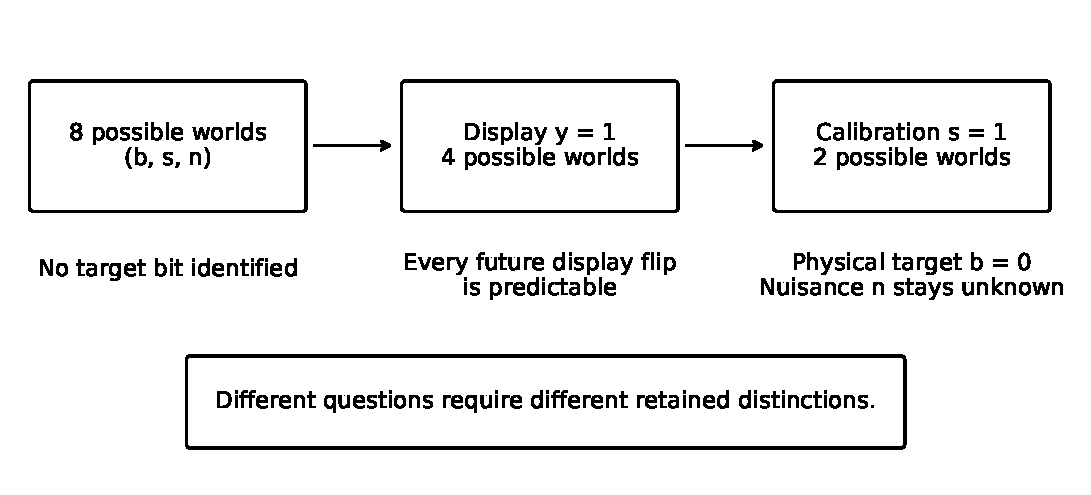
\includegraphics[width=\linewidth]{figures/sensor_chain.pdf}
\caption{One exact observation sequence. The last two worlds differ only in the nuisance bit. Knowing every hidden coordinate is unnecessary for the protected physical target.}
\end{figure}

\section{One answer versus every permitted continuation}
Let $X$ be a finite nonempty state space, and fix an available record $r:X\to H$. Let $\mathcal A$ be a finite alphabet of total deterministic operations $F_a:X\to X$, and let $q:X\to Y$ be the protected output. A word $w=a_1\cdots a_k$ executes $a_1$ first. Thus $F_w=F_{a_k}\cdots F_{a_1}$, and the empty word denotes the identity.

Define behavioral equivalence by
\[
x\sim x'\quad\Longleftrightarrow\quad q(F_wx)=q(F_wx')\text{ for every finite word }w.
\]
The empty word protects the present output. The other words protect its permitted future uses.

\begin{theorem}[Evidence-initialized behavioral state]\label{r:behavior}
A finite predictor initialized only from $r(x)$, updated only by the operation names, and exact for all protected continuation outputs exists if and only if
\[
r(x)=r(x')\ \Longrightarrow\ x\sim x'.
\]
When it exists, $X/{\sim}$ supplies a predictor with the smallest possible number of initialized states. Its updates are $\bar F_a([x])=[F_ax]$ and its readout is $\bar q([x])=q(x)$.
\end{theorem}
\begin{proof}
If two initial records are equal, a deterministic predictor has the same initialized state. Applying the same subsequent operations produces the same predicted outputs. Exactness therefore requires behavioral equivalence.

For the converse, equivalent states have equivalent successors: an output after $F_a$ followed by $w$ is one of the outputs in the defining family. Hence $\bar F_a$ is well defined. The empty word makes $\bar q$ well defined. The fibre premise gives a well-defined initializer $d(r(x))=[x]$. Induction on word length proves exactness. Finally, behaviorally distinct states cannot initialize the same predictor state, since some continuation separates their outputs. Every exact predictor therefore needs at least one initialized value for each class, and the quotient attains that number.
\end{proof}
\source{[GA], Theorem 3.4, and [MU], Theorem 4.1. The two source versions are consolidated, not counted as independent discoveries.}

In the sensor, the display task has two behavioral states. Changing the protected output to $(y,b)$ yields four behavioral states. The old record still has only two values and cannot initialize the enlarged quotient. The new task has exposed a real information requirement.

\section{Why a statistical law is not an observed record}
A parameter can determine a distinct probability law while every finite sample remains possible under several parameters. For instance, Bernoulli parameters $1/3$ and $2/3$ assign positive probability to every finite binary string. No estimator based on one such string can be certainly correct for both parameters. The laws differ, but their finite supports overlap.

A correct uncertainty record can be the appropriate output in this setting. Calling the most probable world ``identified'' would silently replace an error-free claim with a probabilistic one. Chapter~\ref{ch:memory} gives the corresponding probability update explicitly.

\section*{What is now available}
We have a criterion for an initialized predictive state, but no automatic guarantee that an arbitrary coordinate manipulation preserves it. The next chapter studies operations on a representation. Its input is a declared state map and operation family, not an assumed learned encoder.

\chapter{Operations must survive their representations}\label{ch:operations}
\question{A representation is useful only to the extent that its intended operations remain meaningful.}
There are two different ways to change representation. An exact split representation retains the whole mathematical state in another space. A compression retains only part of it. The first can preserve arbitrary composition. The second needs additional conditions.

\section{Exact packets and the hidden-return defect}
Let $V,Z$ be vector spaces over a field. Let $A:V\to Z$ be analysis and $S:Z\to V$ synthesis, with $SA=I_V$. Then $AS$ is an idempotent on $Z$. The map $\mathcal E(T)=ATS$ represents a full-state operator $T:V\to V$ on resolved coordinates. Direct multiplication gives
\[
\mathcal E(T)\mathcal E(U)=ATSAUS=ATUS=\mathcal E(TU).
\]
The resolved identity is $AS$ on the compatible image $A(V)$, not necessarily $I_Z$ on arbitrary coordinates.

For a compression, reverse the splitting. Let $C:V\to Z$ and $R:Z\to V$ satisfy $CR=I_Z$, and put $P=RC$. The compressed operator is $\Phi(T)=CTR$.

\begin{proposition}[Exact accounting of the discarded excursion]\label{r:packet}
For any endomorphisms $T,U$ of $V$,
\[
\Phi(TU)-\Phi(T)\Phi(U)=CT(I-P)UR.
\]
Thus compression preserves this composition precisely when the discarded excursion on the right vanishes. Full split encoding $T\mapsto ATS$ preserves composition without that extra condition.
\end{proposition}
\begin{proof}
Expand the product $\Phi(T)\Phi(U)=CTRCUR=CTPUR$ and subtract it from $CTUR$. The identity for full split encoding follows from $SA=I_V$ as computed above. These computations make no approximation and require no orthogonality.
\end{proof}
\source{Sufficient Resolution [SR], Theorems 2.1 and 2.3. The present proof reviews only these algebraic identities, not the complete forty-seven-page source or its full formal implementation.}

\begin{counterexample}[A discarded coordinate returns]\label{ce:return}
Take $V=\mathbb R^2$, let $C(x_1,x_2)=x_1$, let $R(z)=(z,0)$, and let $T(x_1,x_2)=(x_2,x_1)$. The compressed one-step map is zero. Yet $T^2=I_V$, so $\Phi(T^2)=I_Z$, while $\Phi(T)^2=0$. The discarded second coordinate was not irrelevant to the two-step question.
\end{counterexample}

This is the mathematical reason that a short successful readout is not enough. A representation may preserve what is visible now and lose a route by which hidden information becomes visible later. Packets identify the retained and residual components, but the decomposition alone does not prove the residual harmless.

\section{A method can be transported without reconstructing everything}
Suppose source states $z\in Z$ have operations $F_a$, target states $u\in U$ have operations $G_{\tau(a)}$, and $T:Z\to U$ is a translation. The operation-name map $\tau$ is fixed. Let $q$ and $\bar q$ be matched readouts.

\begin{theorem}[Forward transport of a reusable method]\label{r:transport}
If the source domain is invariant, and
\[
TF_a=G_{\tau(a)}T,\qquad q=\bar qT,
\]
then for every finite word $w$,
\[
TF_w=G_{\tau(w)}T,\qquad qF_w=\bar qG_{\tau(w)}T.
\]
\end{theorem}
\begin{proof}
The empty word gives $TI_Z=I_UT$. Assume the first equality for a prefix. Invariance allows the next local equality to be applied on its successor, yielding
$TF_aF_w=G_{\tau(a)}TF_w=G_{\tau(a)}G_{\tau(w)}T$.
Induction proves the first claim. Composition with the matched readout proves the second.
\end{proof}
\source{[MU], Theorem 6.1. The same local-to-continuation argument appears in OSL and Neuralese. No claim about a learned latent translator is imported.}
\boundary{The theorem is forward. It does not imply an inverse, matching of new target operations, cheap computation of $T$, or that the source solver causally uses the represented state.}

The sensor representation $(y,s)$ translates to $(b,s)$ through $T(y,s)=(y\oplus s,s)$. Flipping the physical bit complements the first coordinate in either representation. The square commutes, and so does every repeated flip. The nuisance bit is never reconstructed because it has no role in this contract.

\section{One quotient for several possible dynamics}
A stronger situation arises when the operator itself is uncertain. Let $V$ be a finite-dimensional vector space over a fixed field, and let $Y$ be a vector space over the same field. Let $T_a^\theta:V\to V$ be a finite family of candidate linear operators indexed by an action $a$ and a model $\theta$. Choose one model $\theta_0$ as the reference and put $A_a=T_a^{\theta_0}$. A model index $\theta$ is fixed during the initial comparison. Let $Q:V\to Y$ be the same linear readout for every candidate.

Define $D_a^\theta=T_a^\theta-A_a$ and the propagated discrepancy space
\[
E=\Span\{A_wD_a^\theta v: v\in V,\ a,\theta,\ w\text{ finite}\}.
\]
It can be constructed by starting with the sum of the discrepancy ranges and repeatedly adding their images under the reference actions. In finite dimension this increasing sequence stops. Immediate invisibility $QD_a^\theta=0$ alone does not guarantee $QE=0$.

\begin{theorem}[A common observable quotient]\label{r:common}
The following conditions are equivalent:
\begin{enumerate}
\item $QT_w^\theta=QA_w$ on all of $V$, for every fixed candidate $\theta$ and every word $w$.
\item $E\subseteq\ker Q$.
\item There is a vector space $Z$, a surjective linear map $r:V\to Z$, common linear updates $G_a:Z\to Z$, and a linear readout $\bar Q:Z\to Y$ with $rT_a^\theta=G_ar$ and $Q=\bar Qr$ for every $a,\theta$.
\end{enumerate}
Under these conditions, $V/E$ is a common quotient and also predicts the output when the candidate index changes between operations.
\end{theorem}
\begin{proof}
Assume the first condition. For every $a,\theta,w$, equality as operators on all of $V$ gives
\[
QA_wD_a^\theta=QT_w^\theta T_a^\theta-QA_wA_a=0.
\]
The last equality applies the premise to the word executing $a$ and then $w$. Spanning proves $E\subseteq\ker Q$.

Conversely, $E$ is invariant under every $A_a$ by construction, and contains the entire range of each difference $D_a^\theta$. Hence $T_a^\theta E\subseteq E$, and every candidate induces the same map $G_a([v])=[A_av]$ on $V/E$. Since $QE=0$, the readout descends. This proves the third condition. Composing its equalities yields the first condition. The same induction permits a different $\theta$ at each step because the quotient map and update remain shared.
\end{proof}
\source{[GA], Theorem 13.1, ``Exact common quotient for structured model uncertainty.'' The all-initial-vectors hypothesis is retained.}

For example, let $Q(x_1,x_2,x_3)=x_1$ and let every candidate act as
\[
T^\theta(x_1,x_2,x_3)=(x_1+x_2,x_2,\theta x_3).
\]
Then $E$ is contained in the third coordinate and remains invisible. The two-coordinate method $(x_1,x_2)\mapsto(x_1+x_2,x_2)$ is exact, although the hidden dynamics are not identified.

The conclusion would be different if a later action moved the third coordinate into the first. That change enlarges $E$ beyond $\ker Q$. It invalidates the use of this quotient, not the theorem that justified the former one.


\section{An algebraic packet is not automatically a probability}
The previous sections concern linear representations. Bayesian correction will require more: a nonnegative state with a well-defined total mass. Those requirements belong to a declared domain, not to the spelling of its coordinates.

Let $\mathcal K$ be a convex cone in a real vector space, and let $\lambda$ be linear and strictly positive on every nonzero member of $\mathcal K$. Its normalized states satisfy $v\in\mathcal K$ and $\lambda v=1$. A coordinate change can send $\mathcal K$ to a cone containing negative coordinates without changing those states' probability meaning. Conversely, an arbitrary signed component of a valid state need not itself be valid.

\begin{proposition}[When complete packets are genuine probability components]\label{r:positive-packets}
Let $P_1,\ldots,P_m$ be linear maps with $\sum_iP_i=I$. If every $P_i$ preserves $\mathcal K$, each normalized $v\in\mathcal K$ has the mixture decomposition
\[
 v=\sum_{i:w_i>0}w_i v_i,\qquad
 w_i=\lambda P_iv\ge0,\quad \sum_iw_i=1,\quad v_i=P_iv/w_i\quad(w_i>0).
\]
Every zero-weight component is zero. If $\mathcal K=\mathbb R^d_{\ge0}$ and the $P_i$ are also idempotent, they must be disjoint diagonal coordinate selections. Orthogonal completeness alone does not imply a probability mixture.
\end{proposition}
\begin{proof}
Cone preservation places $P_iv$ in $\mathcal K$, so its mass is nonnegative. Strict positivity says that a member of this cone with zero mass is zero. Applying $\lambda$ to the complete decomposition gives $\sum_iw_i=\lambda v=1$. Dividing every nonzero component by its mass proves the mixture identity.

On the nonnegative coordinate cone, preservation is equivalent to nonnegative matrix entries, as is seen by applying a matrix to every standard basis vector. Because the matrices sum to $I$, their nonnegative off-diagonal entries must all vanish. An idempotent diagonal entry satisfies $x^2=x$, hence is zero or one. The diagonal sums are one, so each coordinate is selected by exactly one map. Finally, completeness and orthogonality without positivity do not give the first premise, as the following example shows.
\end{proof}
\source{Large Signal Model Foundations [LSM], Proposition 30, physical page 40. Only this finite packet argument and the joint-closure result below are admitted from that source at this stage.}

\begin{counterexample}[An exact detail component has negative probability mass]\label{ce:signed-packet}
For $p=(3/4,1/4)^\top$, the orthogonal average and detail projectors are
\[
 P_{\rm av}=\tfrac12\begin{pmatrix}1&1\\1&1\end{pmatrix},\qquad
 P_{\rm det}=\tfrac12\begin{pmatrix}1&-1\\-1&1\end{pmatrix}.
\]
They sum to the identity and produce $(1/2,1/2)^\top$ and $(1/4,-1/4)^\top$. The components reconstruct $p$ exactly, but the detail has zero total mass without being zero. Normalizing it as a belief is undefined. Clipping its negative entry and normalizing the resulting sum would instead produce $(3/5,2/5)^\top$, a different belief.
\end{counterexample}

\begin{figure}[ht]
\centering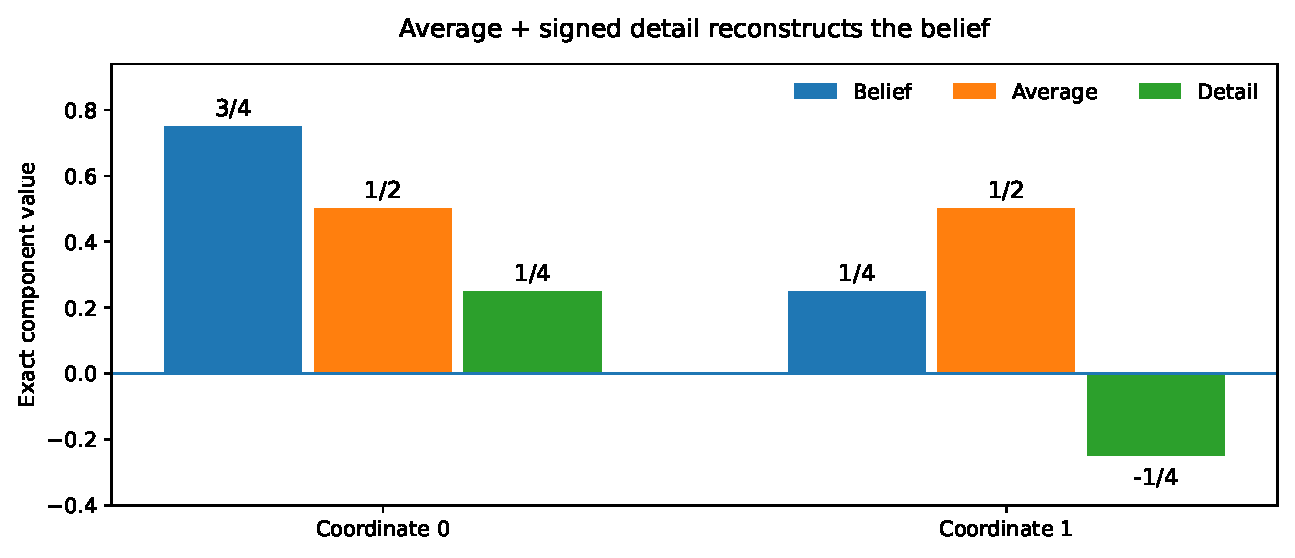
\includegraphics[width=.92\linewidth]{figures/signed_packets.pdf}
\caption{Exact reconstruction and probability interpretation are different requirements. The signed detail is useful algebraically but is not a separate probability distribution. Values are from Counterexample~\ref{ce:signed-packet}.}
\end{figure}

This distinction supplies the interface to the next chapter. A signal packet may describe a discrepancy, a coordinate, or a component of an operator. A belief represents nonnegative mass over alternatives. Moving between them requires a domain-preserving map. No learned signal architecture is inferred from this algebraic admission.

\section*{What is now available}
We have a declared method that preserves the selected outputs. But a predictive quotient need not retain the relationships needed for new evidence. The next chapter changes the retained object from a current physical coordinate to a set or distribution of candidate worlds.

\chapter{Memory that remains open to correction}\label{ch:memory}
\question{A useful memory preserves the distinctions by which its own conclusions can be revised.}
Let $t:\Omega\to Y$ be the current target. A candidate set $V\subseteq\Omega$ records worlds still possible. The empty set is allowed and means that the represented candidates contradict the admitted evidence. It is not a successful identification.

Let $\mathcal E\subseteq\Pow(\Omega)$ contain $\Omega$ and be closed under intersection. In this chapter the world does not change when an evidence event is received. The update is $V\mapsto V\cap E$. Physical actions and their effects will return in Chapter~\ref{ch:inquiry}.

\section{A state sufficient for every later filter}
Define the correction signature
\[
\Sigma(V)=\bigl(t(V\cap E)\bigr)_{E\in\mathcal E}.
\]
It records what each admitted future filter would leave of the possible target values.

\begin{theorem}[Minimal exact memory for a correction contract]\label{r:memory}
Equality of $\Sigma$ is a congruence for every update $V\mapsto V\cap E_0$. The signature supports the current target set and its exact update after every finite evidence sequence. Any deterministic retained state supporting the same readouts and updates on all candidate subsets must distinguish every two distinct signatures. Thus the image of $\Sigma$ has the least possible cardinality for this contract.
\end{theorem}
\begin{proof}
If $\Sigma(V)=\Sigma(W)$, then for each $E$,
\[
t((V\cap E_0)\cap E)=t(V\cap(E_0\cap E))=t(W\cap(E_0\cap E)).
\]
Intersection closure supplies the coordinate $E_0\cap E$, so the updated signatures agree. The $\Omega$ coordinate is the present target set. Induction gives every finite sequence.

If signatures differ, one admitted event produces distinct target sets. A memory that merged those candidates would update identically and return the same answer on that event, contradicting exactness. Hence each signature needs its own state. The signature construction attains the lower bound.
\end{proof}
\source{[GA], Theorem 5.2. This is a behavioral quotient of the correction process, not a claim that all candidate sets must be stored literally.}

\section{An exact count for partition evidence}
Suppose $C_1,\ldots,C_m$ partition $\Omega$ into nonempty cells and the admitted events are \emph{exactly} their unions. Let
\[
D_t=\{(i,y): C_i\cap t^{-1}(y)\ne\varnothing\},\qquad r=|D_t|.
\]
The occupancy memory retains whether a candidate exists in each attainable cell--target pair.

\begin{corollary}[The size of partition correction memory]\label{r:occupancy}
On all subsets of $\Omega$, correction signatures are exactly distinguished by these occupancy records. There are $2^r$ signatures, and $r$ fixed binary bits are necessary and sufficient to encode them.
\end{corollary}
\begin{proof}
An individual-cell filter reveals the target values occupied in that cell, so the signature determines occupancy. Conversely, occupancy determines the target values left by any union of cells. Every subset of $D_t$ occurs: select one world from each included nonempty cell--target intersection and none from excluded intersections. Those intersections are disjoint. Thus there are precisely $2^r$ possible records. The preceding theorem and binary counting give necessity, while the occupancy vector supplies sufficiency.
\end{proof}
\source{[GA], Corollary 5.3. The word ``exactly'' in the evidence premise is essential.}

For this sensor contract, the four cells are fixed pairs $(b,s)$ with either nuisance value. We admit the entire Boolean algebra generated by calibration and display events, including every union of its cells. This is a choice of evidence language, not a claim that a single calibration physically implements every union event. The target is $b$, so there are four attainable cell--target pairs. Candidate membership uses eight bits for eight worlds. Correction memory uses four bits for sixteen possible occupancies. The current target set alone has four possibilities and needs only two bits, but is not sufficient for later calibration.

For example,
\[
V=\{(0,0,0),(1,1,0)\},\qquad W=\{(0,1,0),(1,0,0)\}
\]
have the same possible target set $\{0,1\}$. After the event $s=0$, one leaves target zero and the other target one. Their different associations are operationally relevant.

\begin{counterexample}[A new evidence event changes the required memory]\label{ce:split}
Take one cell $\Omega=\{u,v\}$ and a constant target. The singleton candidate sets have the same old occupancy. If the event $\{u\}$ is added, filtering one singleton gives a target value while filtering the other gives contradiction. A record sufficient for the old event algebra is insufficient for the larger one.
\end{counterexample}

\section{Noisy correction is not elimination}
A likelihood can be small without being zero. Deleting a candidate because an observation was surprising can invalidate a correct noise model. We therefore specify a separate probability contract.

Let $\mathcal M$ be a finite nonempty model set with prior $p(m)$. The sampled model remains fixed during the experiment. For each $m$, let $L_m$ be a probability distribution on a finite nonempty observation alphabet $\mathcal O$. Let $\mathcal Z$ be a finite nonempty report alphabet. A stochastic reporting channel $B(o,z)$, conditionally independent of the model given $o$, creates a retained report $Z\in\mathcal Z$. The joint law is
\[
\Pr(m,o,z)=p(m)L_m(o)B(o,z),\qquad Q_m(z)=\sum_oL_m(o)B(o,z).
\]
Posterior distributions are defined only on positive-probability events.

\begin{theorem}[When a report preserves every Bayesian correction]\label{r:bayes}
The following are equivalent:
\begin{enumerate}
\item For every prior, the posterior after $o$ equals that after $z$ on every positive-probability pair $(o,z)$.
\item The equality holds for one prior positive on every model.
\item There is a stochastic kernel $\rho(o\mid z)$ such that
\[
L_m(o)B(o,z)=Q_m(z)\rho(o\mid z)\quad\text{for all }m,o,z.
\]
\end{enumerate}
The reconstruction in the last condition refers to the actual joint experiment, not an unrelated simulation with matching marginals.
\end{theorem}
\begin{proof}
The first condition implies the second. Under a positive prior, define $\rho(o\mid z)=\Pr(o\mid z)$ whenever $z$ has positive probability. For a positive pair, posterior equality yields
\[
p(m)L_m(o)B(o,z)=\Pr(o,z)p(m\mid o)
=\rho(o\mid z)\Pr(z)p(m\mid z).
\]
Substituting Bayes' formula and cancelling positive $p(m)$ gives the factorization. A zero-probability pair under a positive prior has $L_m(o)B(o,z)=0$ for all $m$. Its conditional weight is zero. If $z$ is impossible for every model, assign any probability row to $\rho(\cdot\mid z)$ because both sides vanish.

Conversely, the factorization makes the likelihood of $(o,z)$ a model-independent multiple of the likelihood of $z$. Normalization under any prior therefore gives $p(m\mid o,z)=p(m\mid z)$. Since the common channel only reads $o$, the same positive-pair posterior equals $p(m\mid o)$. This proves the first condition.
\end{proof}
\source{[MU], Theorem 12.1. The full-support and zero-probability cases are included in the proof.}

The theorem permits removal of an independent nuisance flag. It does not permit removal of every association. Consider two priors on $(b,s)$, with rows indexed by $b$ and columns by $s$:
\[
P=\begin{pmatrix}1/2&0\\0&1/2\end{pmatrix},\qquad
P'=\begin{pmatrix}0&1/2\\1/2&0\end{pmatrix}.
\]
Both individual marginals are uniform. A noisy calibration reports $s$ correctly with probability $3/4$, independently conditional on the fixed world. The probability of report one is $1/2$ under both priors. After that report, however, the target posteriors are $3/4$ and $1/4$. Separate target and sensor marginals cannot support this correction. Their association matters even though neither marginal changed.

These examples do not identify a universally optimal memory. They identify the least information required by a specified correction contract. A new likelihood, a newly admitted model, or a different target can change that requirement.


\section{A record must close under prediction as well as correction}
The preceding Bayesian theorem preserves the posterior over a fixed model family after one experiment. A continuing reasoner also predicts what happens between observations. The same compressed record must support both operations. Otherwise a valid posterior can become an inadequate input to the very next prediction.

First consider a known finite state set $X$ with row-stochastic transition matrices $K_a(x,x')$. We retain column-vector probability distributions. A partition $\pi$ has aggregation $C_\pi(z,x)=1_{\{\pi(x)=z\}}$, so prediction is $p\mapsto K_a^\top p$. For each permitted observation symbol $o$, let $\ell_o(x)>0$ be its specified likelihood. When these are a complete report alphabet, assume also $\sum_o\ell_o(x)=1$.

A mandatory partition $\pi_0$ with at least two blocks protects the target distinctions. We seek a refinement that supports every prediction and each separate Bayesian update for every prior. The observation is an operation available in its own right. This is stronger than inspecting only a chosen combined transition-and-report schedule.

\begin{theorem}[Least refinement closed under prediction and correction]\label{r:joint-refinement}
First split $\pi_0$ by the complete vectors $(\ell_o(x))_o$, obtaining $\pi_{\rm init}$. Then repeatedly split current blocks by
\[
 \left(\sum_{x'\in B}K_a(x,x')\right)_{a,B},
\]
where $B$ runs over the current blocks. The process stops after at most $|X|-|\pi_{\rm init}|$ strict refinement rounds. Its final partition is the unique coarsest refinement of $\pi_0$ for which all specified predictions admit stochastic coarse transitions and all separate Bayesian updates admit fixed strictly positive coarse likelihoods for every prior.
\end{theorem}
\begin{proof}
At a stable partition the probability of reaching each coarse block depends only on the current block. These sums define a stochastic coarse transition and yield $C_\pi K_a^\top=\bar K_a^\top C_\pi$, first on point masses and then by linearity. Likelihoods are constant within final blocks. Grouping the numerator and normalizer by those blocks therefore commutes with every Bayesian update.

For minimality, take any admissible refinement $\eta$ of $\pi_0$. It has at least two blocks. Fix a strictly positive fine likelihood $\ell$ and a strictly positive coarse likelihood $\bar\ell$ inducing its assumed update. For states $x,y$ in one block and $z$ in a different block, compare priors assigning half their mass to $x,z$ and to $y,z$. Their coarse priors agree. Equality of the posterior odds gives
\[
 \ell(x)/\ell(z)=\bar\ell(\eta(x))/\bar\ell(\eta(z))=\ell(y)/\ell(z).
\]
Thus $\ell(x)=\ell(y)$, and $\eta$ refines the first likelihood split. Coarse likelihoods may differ by a positive scale for each observation without changing this conclusion.

If $\eta$ refines a current partition, each current block is a union of $\eta$ blocks. Exact prediction under $\eta$ makes the probability of reaching each such union constant inside every $\eta$ block. Hence $\eta$ refines the next split too. Induction proves that every admissible refinement refines the terminal one. Each strict round increases the block count, proving the bound. Coarseness determines the partition uniquely, up to naming its blocks.
\end{proof}
\source{[LSM], Proposition 9 and Proposition 12, physical pages 11--14. Bayesian necessity also appears in PRIQ [PRIQ], Theorem 5.6. The proof includes the two-block and strict-positivity premises rather than importing them by a cross-reference.}

For the sensor, the mandatory display partition has two blocks. A noisy calibration that reports $s$ correctly with probability $3/4$ splits it into the four $(b,s)$ blocks. The nuisance bit remains merged. The physical flip maps these four blocks among themselves, so the transition stage introduces no further split. The representation is now closed for both prediction and correction, not merely for today's display.

Refinement can also propagate backward through dynamics. In a separate four-state example, the mandatory partition is $\{0,1,2\}\mid\{3\}$ and the deterministic successors are $(0,2,3,3)$. A constant likelihood adds no information. Transition signatures first isolate state 2, then separate 0 from 1. The final partition is discrete. The reason for the second split is a future observable difference, not a newly sampled measurement.

The construction uses complete tables. It does not acquire those tables, certify their physical accuracy, or guarantee a finite encoding of every posterior coordinate. Its least-state statement concerns the specified separate operations and all priors. Different admissible schedules or reachable-prior restrictions can justify another quotient.

\section{Retain the joint law of the report and the next state}
A general experiment can change the state and report correlated information about the change. Describing its transition and report marginals separately is then insufficient. Let
\[
 K_{a,o}(x',x)=\Pr(X_{t+1}=x',O_{t+1}=o\mid X_t=x,A_t=a)
\]
be a nonnegative finite instrument with $\sum_{o,x'}K_{a,o}(x',x)=1$ for every $a,x$. This notation is column-oriented: $K_{a,o}p$ is an unnormalized post-experiment distribution. It specifies an experiment's physical change and its observation in one object.

For a surjection $\pi:X\to Z$, let $C$ sum probabilities over its fibres. Write
\[
 z_{a,o}(p)=\mathbf1^\top K_{a,o}p,\qquad
 \Psi_{a,o}(p)=K_{a,o}p/z_{a,o}(p)
\]
when the denominator is positive. Zero mass means an impossible report under that prior, not an arbitrarily assigned posterior.

\begin{theorem}[One quotient for reports, posteriors, and feedback]\label{r:instrument}
A nonnegative normalized coarse instrument $\bar K_{a,o}$ satisfies
\[
 CK_{a,o}=\bar K_{a,o}C\quad\text{for every }a,o
\]
if and only if, for all $a,o,z'$,
\[
 \sum_{x':\pi(x')=z'}K_{a,o}(x',x)
\]
is constant as $x$ varies within any one input fibre. Such a coarse instrument is unique. Equivalently, it preserves for every prior both the report probabilities and the aggregated positive-probability posteriors:
\[
 z_{a,o}(p)=\bar z_{a,o}(Cp),\qquad C\Psi_{a,o}(p)=\bar\Psi_{a,o}(Cp).
\]
Starting from $Cp_0$, these identities preserve every finite joint action/report law and every corresponding coarse posterior under one common policy that uses only the previously observed action/report history. This includes randomized policies with the same history-conditional action probabilities.
\end{theorem}
\begin{proof}
Applying the matrix identity to a point mass proves necessity of the fibre condition. Conversely, use the common sums to define each column of $\bar K_{a,o}$. They are nonnegative. Summing across $z',o$ partitions the fine successor set and gives column mass one. The definition proves the matrix equality on point masses, hence on every vector. Surjectivity gives uniqueness.

Because $\mathbf1_Z^\top C=\mathbf1_X^\top$, the matrix equality gives equal report masses. Dividing it by a common positive mass gives equal aggregated posteriors. Conversely, equality of masses and positive-mass posteriors gives the unnormalized matrix equality on every prior. If the common mass is zero, both unnormalized vectors are zero by nonnegativity. Point masses finish that direction.

For a history $h$, keep unnormalized states $u_h,\bar u_h$. Initially $\bar u_\varnothing=Cu_\varnothing$. After choosing action $a$ with common probability $\gamma(a\mid h)$ and receiving $o$, the next states are $\gamma(a\mid h)K_{a,o}u_h$ and $\gamma(a\mid h)\bar K_{a,o}\bar u_h$. The intertwining identity preserves their aggregation. Induction gives equal mass for every history, including zero-mass histories. Normalization on positive histories gives the posterior statement. Stopping decisions based on the same history can be included as matching terminal choices.
\end{proof}
\source{Selected synthesis of the positive-transfer and filtering arguments in [PRIQ], Theorems 5.2, 6.1 and 6.3, and the projected-law construction in AVOC [AVOC], Theorem 4.5. The joint instrument and feedback formulation is proved here. No entire nonlinear source theorem or Lean implementation is imported.}

\begin{counterexample}[Correct marginals with an incorrect correction]\label{ce:joint-marginals}
Two fine current states have the same retained label. From the first, the next retained state and report are $(0,0)$ or $(1,1)$, each with probability $1/2$. From the second they are $(0,1)$ or $(1,0)$, again equally likely. In both cases the next-state marginal is uniform and the report marginal is uniform. After report one, however, the next retained state is certainly one in the first case and certainly zero in the second. No common filter based only on the old label can realize both. The joint fibre condition detects exactly the lost association.
\end{counterexample}

Preserving only normalized posteriors is weaker still. A report coin independent of the hidden state leaves every prior unchanged whether its success probability is $1/4$ or $3/4$. Those two instruments have identical posterior maps but different report laws. A planner that prices later branches needs those probabilities. In the exact instrument theorem the evidence scale is fixed, rather than silently discarded during normalization.

\section{Small law error and a rare conditional history}
Approximate models must be compared before declaring their posteriors close. Let $\widetilde K$ be a normalized instrument on the same coarse state and report alphabets. Suppose, at step $t$, every relevant action and fine state satisfy
\[
 \TV\left(\left(\sum_{x':\pi(x')=z'}K_{a,o}(x',x)\right)_{o,z'},
             (\widetilde K_{a,o}(z',\pi(x)))_{o,z'}\right)\le\epsilon_t.
\]
This is a bound on a complete report/next-state distribution, not on an isolated matrix entry. Assume $\TV(Cp_0,\widetilde p_0)\le\delta_0$ with nonnegative $\delta_0,\epsilon_t$. Both models run the same history-based policy. Coarse states recorded in the comparison below are analytical coordinates, not extra observations supplied to that policy.

\begin{proposition}[A whole-history bound with an explicit conditioning cost]\label{r:history-bound}
At horizon $H$, the distributions $P_H,\widetilde P_H$ of the full coarse-state and action/report histories satisfy
\[
 \TV(P_H,\widetilde P_H)\le d_H:=\min\left\{1,\delta_0+\sum_{t=0}^{H-1}\epsilon_t\right\}.
\]
The same bound holds after forgetting any of those history coordinates. For an observed history event $E$ with probabilities $p_E,\widetilde p_E>0$, the conditional final coarse-state distributions obey
\[
 \TV\bigl(P_H(Z_H\in\cdot\mid E),\widetilde P_H(Z_H\in\cdot\mid E)\bigr)
 \le\min\left\{1,\frac{d_H}{\max(p_E,\widetilde p_E)}\right\}.
\]
If either event probability exceeds $d_H$, the other is necessarily positive.
\end{proposition}
\begin{proof}
Condition on a complete coarse history with positive fine probability. Its hidden current-state distribution is a mixture of states in the last coarse fibre. Convexity of total variation makes the true next report/coarse-state row differ from the declared row by at most $\epsilon_t$. Mixing over a common action kernel preserves this bound. Extend the two old history laws first through the same declared row. Total variation cannot increase under a common stochastic kernel, by the triangle inequality and row sums. Replacing those rows with the true conditional rows adds at most $\epsilon_t$, weighted by a total history mass of one. Hence the history distance at the next step is at most the old distance plus $\epsilon_t$. Induction and the cap one prove the first claim. Summing over forgotten coordinates is also a stochastic map, proving the second.

For conditioning, let $u,v$ be the restrictions of the two history laws to $E$, with masses $p_E,\widetilde p_E$. The difference on the complement has $\ell^1$ norm at least $|p_E-\widetilde p_E|$. Thus
\[
 \|u-v\|_1+|p_E-\widetilde p_E|\le2d_H.
\]
Adding and subtracting $v/p_E$ bounds the conditional distance by $d_H/p_E$. Interchanging the laws gives $d_H/\widetilde p_E$, so the smaller of these bounds has the displayed maximum denominator. Projection to the final state cannot increase the distance. Finally, the probability of any event changes by at most total variation, which proves positivity when one mass exceeds $d_H$.
\end{proof}
\source{Finite probability-instrument specialization of [LSM], Propositions 43--44, with the joint retained-state record made explicit. The symmetric conditioning form follows by applying the same elementary bound in both directions. [PRIQ], Section 9 supplies the complementary stepwise posterior-error perspective.}

\begin{counterexample}[A rare report carries the entire discrepancy]\label{ce:rare-history}
Two joint laws place mass $1-\delta$ on the same ordinary outcome. On a report event $E$ of mass $\delta>0$, one puts all mass on retained state zero and the other on retained state one. Their whole-law distance is $\delta$, while their conditional distance after $E$ is one. The factor involving event probability is therefore essential. This is a finite-law statement, not an empirical estimate of a sensor error.
\end{counterexample}

\begin{figure}[ht]
\centering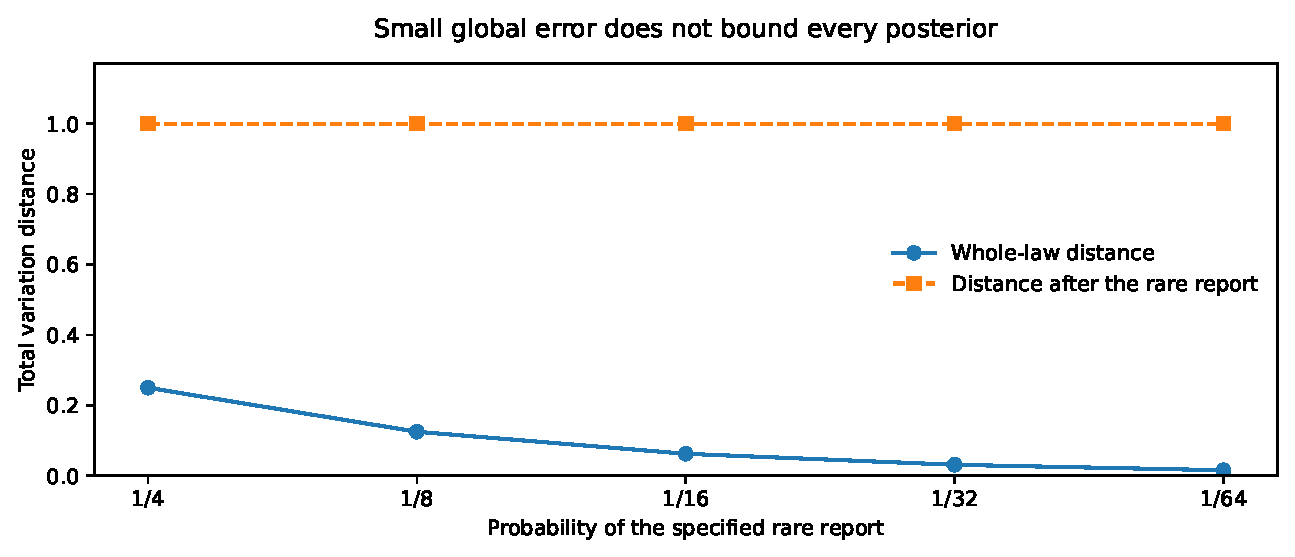
\includegraphics[width=.92\linewidth]{figures/rare_history.pdf}
\caption{In Counterexample~\ref{ce:rare-history}, shrinking the rare-event mass reduces whole-law error but leaves conditional error maximal. The points are exact specified probability laws, not sampled observations.}
\end{figure}

The bound compares one policy across two models, not independently optimized controllers. Chapter~\ref{ch:inquiry} supplies the uniform comparison needed for re-optimization. First, the next chapter asks what decisions and explanations the corrected record can justify.

\chapter{From corrected records to decisions and explanations}\label{ch:decision}
\question{The same record, model, and continuation must support the decision being certified.}
Correctness of a probability calculation is not a guarantee that a real process follows its likelihood model. Within the declared model, however, a small error in the retained distribution can support a precise decision bound. We state that bridge before introducing communication, so that an explanation has a definite object to preserve.

\section{One quantitative decision contract}
Let $p$ and $\widehat p$ be distributions on the same finite world set. For each world let $v_\omega$ be a response and $\widehat v_\omega$ its approximation in one metric space. Assume
\[
\TV(p,\widehat p)\le e,\qquad
\sup_\omega d(v_\omega,\widehat v_\omega)\le d_0.
\]
For each action $a$ in a finite nonempty set, let the loss $\ell(a,v)$ lie in $[0,1]$ and be $K$-Lipschitz in $v$. Define the model risks
\[
R(a)=\sum_\omega p(\omega)\ell(a,v_\omega),\qquad
\widehat R(a)=\sum_\omega\widehat p(\omega)\ell(a,\widehat v_\omega).
\]

\begin{theorem}[A decision bound for one actual approximation chain]\label{r:risk}
Put $\xi=\min\{1,e+Kd_0\}$. For every action, $|R(a)-\widehat R(a)|\le\xi$. If $\widehat a$ minimizes the approximate risk, then
\[
R(\widehat a)-\min_a R(a)\le\min\{1,2\xi\}.
\]
If the approximate gap between its unique minimizer and every alternative exceeds $2\xi$, that action is also the unique true model-risk minimizer.
\end{theorem}
\begin{proof}
Add and subtract $\sum_\omega p(\omega)\ell(a,\widehat v_\omega)$. The response term has absolute value at most $Kd_0$. The expectation of a function in $[0,1]$ changes by at most total variation, giving the other term at most $e$. Risks lie in $[0,1]$, so their difference is also at most one.

For a true minimizer $a_*$,
\[
R(\widehat a)\le\widehat R(\widehat a)+\xi
\le\widehat R(a_*)+\xi\le R(a_*)+2\xi.
\]
The loss range supplies the cap one. Finally, for any other $a$, subtract the two error bounds to obtain
$R(a)-R(\widehat a)\ge\widehat R(a)-\widehat R(\widehat a)-2\xi>0$.
\end{proof}
\source{[GA], ``A common quantitative grounding certificate'' and [MU], ``A joint posterior and recipient decision certificate.'' This is a specialization to a common finite candidate set and bounded loss.}

The phrase ``model risk'' matters. The theorem cannot repair an omitted candidate, a false sensor convention, or an action outside the stated loss function. It also cannot combine a posterior bound from one history with a response bound from another. The record must bind the actual calculation and its premises.

For the noisy calibration example, use zero-one loss for selecting the target bit. Under $P$ and report one, choosing one has risk $1/4$, while choosing zero has risk $3/4$. An approximation with total variation at most $1/10$ and no response error preserves the unique decision because the gap $1/2$ exceeds $2/10$. Under $P'$ the correct decision reverses. A valid error bound around the wrong prior is not a substitute for retaining the correct association.

\section{An explanation belongs to a recipient}
An artifact is not an explanation merely because its producer can interpret it. Fix a finite case set $X$, a sender-access map $\alpha:X\to H$, and a finite artifact catalogue $\mathcal C$. Recipient $i$ has a background record $\beta_i(x)$, a demanded output $t_i(x)$, and a fixed bounded procedure $L_i$. A timeout, malformed artifact, wrong output, or budget overrun counts as failure.

Let $\mathcal C(x)$ be the artifacts that succeed for every recipient in case $x$. For an attained sender value $h$, put
\[
\mathcal C_h=\bigcap_{x:\alpha(x)=h}\mathcal C(x).
\]

\begin{theorem}[A common artifact for fixed recipients]\label{r:recipient}
A sender restricted to $\alpha(x)$ can provide one exact artifact for all recipients if and only if every $\mathcal C_h$ is nonempty. When feasible, the smallest possible number of distinct transmitted artifacts is
\[
\min\{|C|:C\subseteq\mathcal C,\ C\cap\mathcal C_h\ne\varnothing
\text{ for every attained }h\}.
\]
\end{theorem}
\begin{proof}
A sender seeing $h$ must choose the same artifact for all cases in that fibre. It must therefore select a member of $\mathcal C_h$, proving necessity. Choosing one member of each nonempty finite intersection gives a valid encoder. The image of any encoder intersects every $\mathcal C_h$. Conversely, any catalogue meeting all those sets supplies such an encoder by choosing from the intersections. Finite minimization gives the formula.
\end{proof}
\source{[MU], ``The fixed-recipient covering criterion.'' The earlier designed-decoder coloring criterion is not substituted for the installed-recipient problem.}

\begin{counterexample}[Individual acceptability is not a common message]\label{ce:message}
Two cases have the same sender record. In one, the sole acceptable artifact is $c_0$. In the other it is $c_1\ne c_0$. Each case has a valid explanation if its hidden identity is known. Their intersection is empty, so the sender cannot select a valid common explanation from its actual information.
\end{counterexample}

In the sensor, a sender observing $y$ can transmit one bit to a recipient holding $s$. The recipient's fixed XOR procedure returns $b=y\oplus s$. The sender need not know $b$: its message combines with the recipient's background.

A decoder that ignores this message fails where background alone cannot distinguish the target. More strings do not fix that procedure. Installed information, interpreter work, and message size are separate resources.

\chapter{One investigation, one resource budget}\label{ch:inquiry}
\question{A possible answer, an affordable observation, and a small program must belong to the same workflow.}
Let $X$ be a finite nonempty state space. It includes every origin tag, permission, background record, and history variable that affects the stated behavior. An experiment $e$ is allowed on a domain $D_e\subseteq X$, has a deterministic successor $f_e:D_e\to X$, a report $o_e:D_e\to O_e$, and a fixed nonnegative integer resource vector $c_e$.

A current support $V\ne\varnothing$ records possible states. The experiment is permitted only if $V\subseteq D_e$. After report $o$, the possible \emph{post-experiment} states are
\[
V_{e,o}=\{f_e(x):x\in V,\ o_e(x)=o\}.
\]
Only nonempty report branches are retained. If the target concerns a past value, that value must survive as an immutable tag. Resetting the current state is not recovering its history.

The experiment catalogue and the terminal-artifact catalogue are finite, and the resource vector has a fixed finite dimension. A terminal artifact $a$ is acceptable only if every fixed recipient succeeds in every state of $V$. Its worst-case terminal cost is $g_a(V)$, computed componentwise. A controller is a literal finite tree with one record per experiment or terminal node. Stored memory counts all branches, including those not visited in one execution.

\section{The complete finite frontier}
Let $\mathcal P_h(V)$ be the nondominated pairs $(v,m)$ of worst-case online resource vectors and stored-record counts attainable by successful trees with at most $h$ experiment steps. At depth zero the available pairs are
\[
\operatorname{Pareto}\{(g_a(V),1):a\text{ succeeds throughout }V\}.
\]
At greater depth retain those stops and, for each uniformly permitted experiment and one feasible child pair $(v_o,m_o)$ for every nonempty branch, form
\[
\left(c_e+\max_o v_o,\quad1+\sum_o m_o\right).
\]
A profile dominates another when it is no larger in every resource coordinate and strictly smaller in at least one. The maximum is componentwise. An impossible child contributes no tree. It is not a zero-cost branch.

\begin{theorem}[Exact joint feasibility for explicit controllers]\label{r:inquiry}
This recurrence gives exactly the nondominated resource profiles of successful depth-bounded controllers. Every retained pair has a concrete tree witness. A common online and storage budget is feasible if and only if it bounds one retained pair. Removing dominated child profiles does not change feasibility under any componentwise budget.
\end{theorem}
\begin{proof}
At zero depth the only possibilities are acceptable terminals, whose profiles are exactly the stated stops. At positive depth a successful tree either stops or begins with one uniformly allowed experiment. Every possible report needs a successful child on precisely $V_{e,o}$. By induction those children have profiles in the lower-depth attainable set. Worst-case online cost is the root cost plus their componentwise maximum. Complete tree storage is one plus the sum of all child records.

Conversely, combining any allowed root with a successful child for every report constructs a successful tree with that profile. This proves exact enumeration before pruning. Replacing a dominated child by a dominating one cannot increase either a coordinatewise maximum or a sum of record counts, and does not change its supported initial set. Thus Pareto pruning preserves every feasible budget and every retained profile has a witness.
\end{proof}
\source{[MU], ``A joint resource certificate for fixed recipients,'' and [SII], Theorem 6.2. The scalar-cost repair case is a specialization, not a different composition theorem.}

The recurrence can be expensive. It is a finite mathematical characterization, not an efficient general learner. It assumes its transition and acceptance tables. Their discovery and checking are preparation costs, not free consequences of the existence theorem.

\begin{counterexample}[Two separate optima do not form one controller]\label{ce:pareto}
There are four immutable cases, each requiring its own terminal answer. A direct observation of the case costs four units and gives a five-record tree including four terminals. Unit-cost equality tests can identify the case in at most three tests with seven records. Terminal answers have zero online cost in this particular example. The frontier is $(4,5)$ and $(3,7)$. The mixed budget $(3,5)$ is infeasible: an all-equality successful tree needs four leaves and at least seven records. Any tree using the direct observation on a reachable path costs at least four.
\end{counterexample}

\begin{figure}[ht]
\centering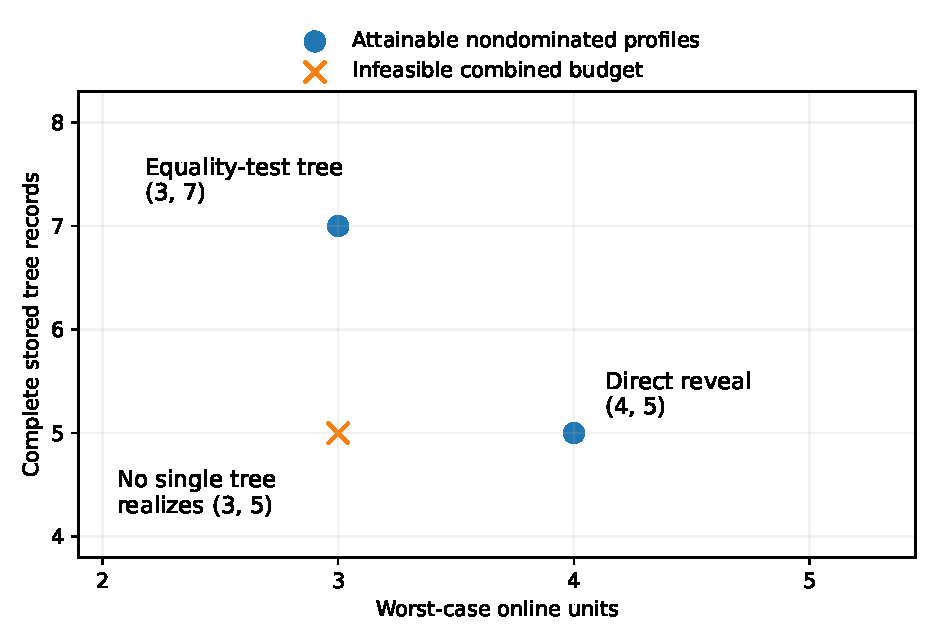
\includegraphics[width=.88\linewidth]{figures/joint_frontier.pdf}
\caption{The four-origin example has two nondominated profiles. Combining the lowest coordinate from each does not construct a feasible controller. Terminal answers have zero online cost in this example.}
\end{figure}

\section{When a checked candidate can end the search}
Consider $n\ge1$ immutable cases with total nondestructive binary unit-cost queries. Every unit-cost repair succeeds in exactly one case, and every case has a repair. A controller must succeed certainly in every case.

\begin{theorem}[A candidate attaining both lower bounds is optimal]\label{r:lowerbound}
Every successful controller has worst-case work at least $1+\lceil\log_2n\rceil$ and literal storage at least $2n-1$. A checked controller attaining both bounds and the requested horizon realizes the entire nondominated work/storage frontier.
\end{theorem}
\begin{proof}
Distinct cases cannot end at the same successful repair leaf, so at least $n$ leaves are reachable. A binary tree of query depth $d$ has at most $2^d$ leaves, giving $d\ge\lceil\log_2n\rceil$. The terminal repair adds one unit.

Let $l$ be the number of leaves and $i_1,i_2$ the counts of unary and binary internal nodes. Counting tree edges gives $i_1+2i_2=i_1+i_2+l-1$, hence $i_2=l-1$. Total records are $2l-1+i_1\ge2n-1$. A successful candidate at both coordinatewise lower bounds dominates every other attainable cost profile. Its validity and horizon check make it an actual member of the frontier, leaving that pair as the whole nondominated frontier.
\end{proof}
\source{[SII], Theorem 11.1. The assumptions exclude destructive resets and repairs that succeed on several cases.}

For eight possible defective cells, equality-first diagnosis requires seven queries in the worst case, while three coordinate-bit queries identify the cell. Including repair gives costs eight and four, respectively. Both literal trees have fifteen records. Faster execution has not eliminated the cost of storing the procedure.

This eight-cell example is separate from the eight-world sensor. The sensor has only four action-relevant $(b,s)$ pairs and an irrelevant nuisance coordinate. Confusing hidden-world cardinality with the number of required repair distinctions would import a false lower bound.


\section{Expected-cost inquiry uses the report probabilities}
The preceding frontier certifies worst-case execution and complete tree storage for deterministic observations. A noisy report requires a different optimization. Expected cost weights each future branch by its probability. A low expectation is not a hard execution budget, and neither replaces the cost of storing the whole controller.

Use the finite instrument of Theorem~\ref{r:instrument}, with fine belief $p$ and coarse belief $q=Cp$. At $q$, a finite set of experiments $A(q)$ is permitted, and a nonempty finite set of terminal decisions $D(q)$ is available. These catalogues must be identical for every fine belief with the same $q$. Stopping with decision $d$ has loss $\ell_d(\pi(x))$ in fine state $x$, so its conditional risk is $\langle q,\ell_d\rangle$. An experiment has a finite nonnegative charge $c_a(q)$, identical on the fine and coarse side. All history variables affecting permissions, charges, or targets must be included in the declared state.

Let $J_h(p)$ be the least expected charge plus terminal loss attainable using at most $h$ further experiments, with terminal decisions permitted at any step. It is defined by finite observation trees, not by a hidden-state controller. Its coarse recurrence is
\begin{align*}
 \bar J_0(q)&=\min_{d\in D(q)}\langle q,\ell_d\rangle,\\
 \mathcal Q_h(q,a)&=c_a(q)+\sum_{o:\bar z_{a,o}(q)>0}
       \bar z_{a,o}(q)\bar J_{h-1}\bigl(\bar\Psi_{a,o}(q)\bigr),\\
 \bar J_h(q)&=\min\left\{\bar J_0(q),\ \min_{a\in A(q)}\mathcal Q_h(q,a)\right\}.
\end{align*}
An empty experiment catalogue leaves only stopping. Impossible reports do not receive invented posteriors.

\begin{theorem}[The same compressed belief supports the same inquiry]\label{r:belief-planning}
Under the exact instrument quotient and the common loss, charge, and catalogue assumptions above,
\[
 J_h(p)=\bar J_h(Cp)\quad\text{for every prior and every finite }h.
\]
Every first-action value and optimal first-action set agrees. A minimizing coarse-belief policy produces a fine-model optimal history-based policy, including its stopping decision. Finite minimizing trees exist. The result supplies neither an efficient synthesis algorithm nor a worst-case storage or resource guarantee.
\end{theorem}
\begin{proof}
At zero horizon the terminal risks agree by fibrewise summation. Suppose the equality holds at $h-1$. For any permitted first experiment, Theorem~\ref{r:instrument} gives the same probability of each report and the same coarse posterior on every positive branch. The induction hypothesis gives equal optimal continuation costs on each such branch. The first charge agrees, so the entire action value agrees. Stopping has the same value as well. Taking the minimum over the identical catalogues proves both value equality and equality of minimizing first choices.

Choose one minimizing first choice and attach minimizing lower-horizon trees to its finitely many positive branches. If the choice is terminal, no child is required. Induction constructs a finite tree attaining the value. The same induction bounds every other admissible tree below by that minimum. An observed history initializes the same coarse belief in the fine execution, so selecting from that belief realizes the coarse policy without observing the fine hidden state.
\end{proof}
\source{The finite backup and projected-law proof mechanisms of [AVOC], Theorems 4.5 and 9.2, applied here to the belief transition supplied by Theorem~\ref{r:instrument}. The source-facing Machine Theory correspondence covers this selected result. That correspondence is separate from any claim that the complete AVOC implementation is verified. The established partially observed planning context is [KLC].}

\begin{counterexample}[A correct probability quotient can hide a forbidden action]\label{ce:permission-loss}
Two fine states share all report and transition probabilities and are given the same coarse label. A terminal repair is permitted in one state but forbidden in the other. The instrument quotient is valid, but a coarse interface that offers the repair in both states is not. Exact belief and value formulas do not repair a missing permission distinction. The catalogues must factor through the retained state, or the state must be refined.
\end{counterexample}

\section{The sensor chooses when another calibration is worth its cost}
Return to the sensor after display $y=0$. Conditional on that display, assign equal probability to $(b,s)=(0,0)$ and $(1,1)$, with any nuisance distribution inside each pair. Only noisy calibration and terminal bit selection are offered in this example. A calibration reports $s$ correctly with probability $3/4$, with fresh conditionally independent noise and no change to the hidden world. It costs $1/20$ in the same stated loss units as a wrong terminal choice, whose loss is one. A correct terminal choice has loss zero.

The retained belief on the four $(b,s)$ pairs is an exact quotient of the eight-world belief. Its two diagonal masses initially equal $1/2$. After one calibration the favored target has probability $3/4$. A second matching report raises that probability to $9/10$, while conflicting reports restore $1/2$.

\begin{center}\begin{tabular}{@{}>{\raggedright\arraybackslash}p{.16\linewidth}>{\raggedright\arraybackslash}p{.24\linewidth}>{\raggedright\arraybackslash}p{.54\linewidth}@{}}\toprule
Report limit & Optimal expected cost & An optimal initial choice\\\midrule
0 & $1/2$ & Stop and select either bit.\\
1 & $3/10$ & Calibrate once, then select.\\
2 & $3/10$ & Calibrate once, then stop.\\
3 & $11/40$ & Calibrate, then use an adaptive continuation.\\\bottomrule\end{tabular}\end{center}

\begin{figure}[H]
\centering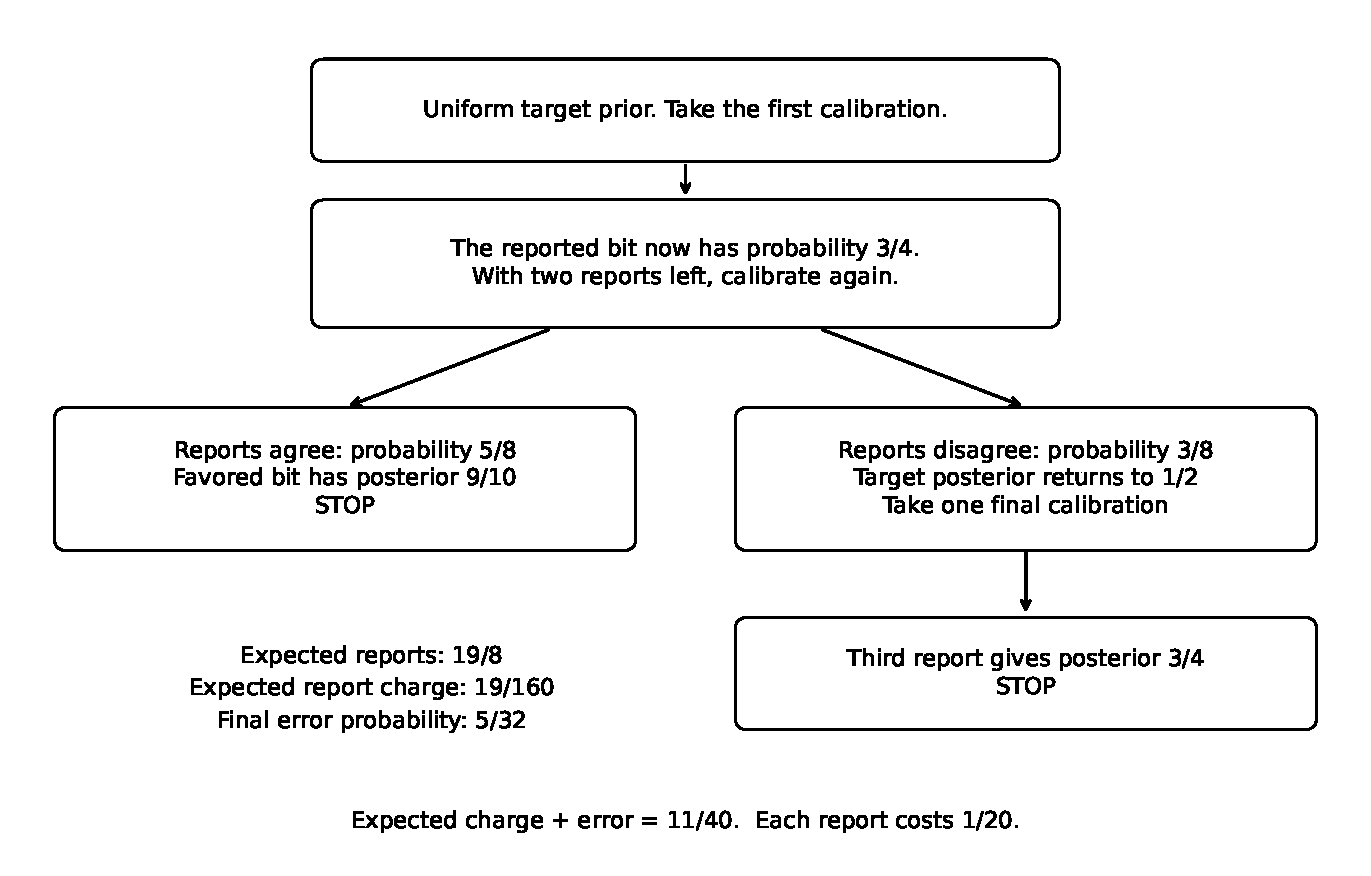
\includegraphics[width=.94\linewidth]{figures/calibration_policy.pdf}
\caption{An optimal three-report policy in the unchanged eight-world sensor with the explicitly added noisy calibration channel. All masses and costs are exact. The diagram groups sign-symmetric report histories, not distinct hidden states supplied to the agent.}
\end{figure}

With three reports available, the optimal policy takes a second report after the first. If the first two agree, it stops. If they disagree, it takes the third. The disagreement probability is $3/8$. Thus the expected report count is $2+3/8=19/8$, the expected charge is $19/160$, and the error probability is $5/32$. The total is $19/160+5/32=11/40$.

A second report alone does not reduce expected classification error enough to pay for itself. A third-report allowance makes it worthwhile to investigate only the unresolved branch. This gain is achieved by one contingent policy, without access to the hidden bit.



The two-valued display state is too coarse for this inquiry. The four-pair probability record supports calibration and decisions while still discarding the nuisance bit.

\section{An approximate model supports a different, quantitative claim}
Exact policy transport and approximate planning must not share one unqualified guarantee. Fix a finite horizon $H$ and one nonempty finite class $\mathfrak P$ of admitted action/report trees, shared by the true and approximate models. The complete loss of a tree is the same function of its coarse-state and action/report path in both models, taking values in $[0,B]$. For example, a terminal loss in $[0,1]$ and at most $H$ charges bounded by $c_{\max}$ give $B=1+Hc_{\max}$.

Assume Theorem~\ref{r:history-bound}'s bound $d_H$ holds uniformly over every tree in that class. An early stop is padded by a common absorbing terminal step for the history comparison. State-dependent charges are permitted when included in the same coarse-path loss. A model-dependent posterior score used as an uncharged surrogate loss would be a different problem.

\begin{proposition}[Uniform model error controls a changed policy]\label{r:policy-error}
Let $J(\pi)$ and $\widetilde J(\pi)$ be a tree's expected losses in the true and approximate models. Then
\[
 |J(\pi)-\widetilde J(\pi)|\le Bd_H\quad(\pi\in\mathfrak P).
\]
If $\widetilde\pi$ minimizes the approximate loss and $\pi_*$ minimizes the true loss over this same class, then
\[
 J(\widetilde\pi)-J(\pi_*)\le\min\{B,2Bd_H\}.
\]
These conclusions do not certify a zero-risk constraint or preservation of admissibility outside the common class.
\end{proposition}
\begin{proof}
The expectation of a function in $[0,B]$ changes by at most $B$ times total variation. Apply the common-policy history bound separately to each fixed tree, proving the first assertion uniformly. Now
\[
 J(\widetilde\pi)\le\widetilde J(\widetilde\pi)+Bd_H
 \le\widetilde J(\pi_*)+Bd_H\le J(\pi_*)+2Bd_H.
\]
The loss range gives the cap $B$. Each tree is first compared with itself across models, before applying optimality to different controllers. A zero-probability bad event in one model can have positive probability in the other, so the average bound does not certify sure feasibility.
\end{proof}
\source{Direct combination of the whole-history bound with the selection argument already used in Theorem~\ref{r:risk}. [AVOC], Sections 8--10, provide the source context for guarded planning and model-error value bounds. This finite fixed-policy-class formulation is stated and proved in full here.}

With true calibration accuracy $37/50$ and planning accuracy $3/4$, the one-step defect is $1/100$. Taking $H=3$ and $B=23/20$ gives the uniform regret bound $69/1000$. A computed performance value does not replace that guarantee. Expected-risk and hard-budget claims remain distinct.

\chapter{Improving discovery without changing its meaning}\label{ch:discovery}
\question{Removing redundant work is an improvement only when the removed work could not change the justified result.}
Let $\mathcal G=(p_0,\ldots,p_{N-1})$ be a finite ordered grammar of pure, total candidate programs. Let $D$ be a finite context set and $t:D\to Y$ a fixed labeling. A teacher either accepts a candidate that agrees everywhere or returns a context where it disagrees. The teacher's work is part of the development account.

\section{Finite counterexample-guided acquisition}
The learner retains every returned counterexample. It proposes the earliest candidate consistent with all retained examples, or reports exhaustion of the grammar when none remains.

\begin{proposition}[What finite counterexamples establish]\label{r:cegis}
The learner never submits the same rejected candidate twice. Within at most $N$ teacher calls, it returns the earliest globally correct candidate in the declared grammar or exhausts that grammar. A timeout before this process finishes is neither acceptance nor exhaustion.
\end{proposition}
\begin{proof}
Each counterexample refutes the submitted program and remains a constraint forever. That program cannot be submitted again. A globally correct candidate never violates a truthful counterexample. With only $N$ candidates, either an accepted one is found or all are ruled out. If the accepted candidate were preceded by a globally correct candidate, that earlier candidate would still be consistent and would have been selected first. This proves the ordering claim. Interruption changes none of these logical implications and cannot supply a completed search result.
\end{proof}
\source{[SII], Theorem 15.1. This is finite exact synthesis in a supplied language, not a statistical generalization guarantee.}

Agreement on $D$ is not validity outside $D$. That distinction is especially important when a candidate is used to prune future searches. A wrong proposal can be rejected by a final checker. A wrong pruning rule may remove the only candidate the checker ought to see.

\section{A learned search representation can preserve the exact investigation}
Suppose a deterministic normalizing map $n$ is sound in the following direction:
\[
n(p)=n(q)\ \Longrightarrow\ p(z)=q(z)\quad\text{for every admitted context }z.
\]
The map need not detect every semantic equivalence or produce a mathematically canonical normal form. Each successful contextual rewrite must be justified under the actual pure, total semantics. Keep the earliest original AST for every attained normal form, not a replacement AST with an uncharged new interpreter.

\begin{theorem}[Ordered semantic compression preserves the teacher trace]\label{r:ordered}
Assume all counterexamples are retained, candidate and example orders are fixed, and the teacher is deterministic and extensional, returning the first disagreement in a fixed context order. Searching only the earliest representatives yields exactly the same submitted ASTs, counterexamples, and final acceptance or grammar exhaustion as the original learner. With the same AST interpreter it uses no more retained-example evaluations. Preparation, dispatch, and stored-index costs are separate.
\end{theorem}
\begin{proof}
A removed expression has an earlier representative with the same values on every admitted context. If that representative was accepted, the original search ended before reaching the removed expression. Otherwise an already retained example refuted the representative, either during a consistency test or from the teacher. Persistence of examples means that the same example refutes the later equivalent expression. The original learner therefore never submits that removed expression to the teacher.

Deleting only those unsuccessful consistency tests preserves the next submitted AST. A deterministic teacher then returns the same counterexample or acceptance. Induction over submissions proves equality of the complete trace, including exhaustion. Every deleted evaluation has nonnegative cost in the named evaluation count. The argument makes no claim that constructing or consulting the representative index is free.
\end{proof}
\source{[SII], Theorems 21.1 and 21.2. Sound equational replacement is the premise. Empirical agreement on a few probe points does not supply it.}

\begin{counterexample}[A probe-equivalent equation is not a general identity]\label{ce:probe}
The expressions $\max(x,1)$ and $x$ agree for probes $x\in\{1,2,3\}$. At zero they differ. Grouping them by those probe values alone can remove a needed candidate. The identity $\max(x,0)=x$ is valid over nonnegative integers, but not over all integers. The semantic domain is part of the equation's certificate.
\end{counterexample}

The retained object may therefore improve later search without containing its answers. This is the precise process-level role of a checked equation library. The grammar, primitive semantics, teacher, and proof rules can still be supplied. Their presence must remain visible instead of being redescribed as discoveries.

\section{A reusable rule for stopping an unpromising read}
A diagnostic compiler inspects a binary query on $m$ immutable cases. In the prefix already read, $a$ cases give zero and $b$ give one. Each child is allowed at most $C$ cases because the remaining binary depth has that leaf capacity. Assume integers
\[
C\ge1,\quad 2\le m\le2C,\quad a,b\ge0,\quad a+b\le m.
\]

\begin{proposition}[A sound prefix exclusion]\label{r:prefix}
The unread reports can be completed with both final branch counts at most $C$ if and only if $\max(a,b)\le C$. A scan may therefore stop when one count first exceeds $C$. In a fixed ordered depth-first compiler with identical scope, terminal, and fallback rules, replacing full root scans by this early rejection preserves the first returned tree or the completed depth-bounded failure result.
\end{proposition}
\begin{proof}
Counts only increase, so an overfull child cannot be rescued. Otherwise the two remaining capacities are $C-a$ and $C-b$, both nonnegative. Their sum $2C-a-b$ is at least the number $m-a-b$ of unread rows. Distributing the unread cases between those capacities gives a feasible completion.

Every root rejected early would also be rejected after its full scan. A root not rejected early is read completely and produces the same ordered child supports. Induction on the finite remaining depth therefore yields identical recursive searches, backtracking, and first completion. The same failure condition invokes the same fallback. The skipped rows are only suffixes whose contents could not change rejection. A resource timeout is excluded from the completed-failure claim.
\end{proof}
\source{[SII], Proposition 16.1 and Theorem 16.3. The conclusion concerns capacity feasibility, not the existence of a completing query in the installed language.}

For $C=4$, a fifth zero already closes a root. Reading more rows cannot reduce that branch. By contrast, a four-versus-four split merely survives this necessary test. If no remaining query distinguishes either child, the root still fails.

\begin{counterexample}[A changed repair defeats the old premise]\label{ce:universal}
Four cases previously required four different repairs. Admit one new repair successful in all four. No identifying query is now needed. The old singleton-leaf lower bound and its pruning interpretation are not applicable. The correct response is to recheck the repair scope, not to preserve an obsolete optimization because it once passed.
\end{counterexample}

\section*{What is now available}
The resulting method is semantically justified only under its premises. We must still determine whether it saves total resources, and which proof records remain usable when a later revision changes those premises. Both questions belong to the next chapter rather than being inferred from a successful synthesis.

\chapter{What remains valid after a revision}\label{ch:revision}
\question{A mathematical proof can remain true while no longer applying to the installed system.}
A certificate for ordinary integer addition is not a certificate for an operation with the same printed name and a different implementation. A grammar quotient depends on the grammar order. A comparison depends on the actual controller and the prices used to value its events. These are distinct dependencies.

\section{Reuse follows semantic dependencies}
Let an artifact state be $a=(a_1,\ldots,a_d)$. A finite directed acyclic graph represents claimed guarantees. For vertex $v$, let $D_v$ be its direct artifact dependencies and let $\operatorname{pa}(v)$ be its parent guarantees. The declaration is semantically complete if the meaning of its claim and local verification rule is determined by those components and parent claims. External assumptions are included explicitly as premises.

After changing $a$ to $a'$, mark a vertex stale when a direct input changes and propagate staleness to all descendants. Call the resulting set $\Delta$.

\begin{theorem}[Selective reuse with complete dependencies]\label{r:dependencies}
Assume the graph is finite and acyclic, direct dependencies are semantically complete, local rules are sound, and the applicable external premises hold. Assume also that every old witness established its old claim before the revision. Old witnesses still establish every claim outside $\Delta$. Re-establishing affected claims in topological order, using revised values and established parents, restores the corresponding revised claims. Without an affected parent's re-establishment, this reuse rule supplies no justification for its dependent claim.
\end{theorem}
\begin{proof}
A vertex outside $\Delta$ has unchanged direct values and no stale parent. In topological order, induction shows that every parent retains its meaning and proof. Completeness of the dependency declaration leaves the local argument applicable. For a stale vertex, once its revised parents are established, soundness of the newly checked local rule gives the revised conclusion. A second topological induction proves restoration. An unchecked parent leaves a missing premise, so the rule alone cannot justify a dependent conclusion. This is not a proof that the conclusion is false.
\end{proof}
\source{[SII], Theorem 24.1. It is a theorem about a declared complete dependency graph, not a method that infers complete dependencies from arbitrary programs.}

\begin{counterexample}[A missing dependency defeats a perfect replay]\label{ce:dependency}
A stored claim is $u=v$, initially with both values zero. Its registry records only $u$. Change $v$ to one. A flawless comparison with the recorded $u$ still passes, while the claim is false. A hash or replay cannot recover the premise the registry omitted.
\end{counterexample}

Adding the universal repair from the preceding chapter changes a successful-repair set. It invalidates a cardinality certificate and any dependent performance statement. It need not invalidate an arithmetic equation used elsewhere. A new valid repair also does not inherit the old controller's speed comparison. Rechecking can legitimately conclude that the new route is slower, cheaper, or incomparable under the stated resources.

\begin{figure}[ht]
\centering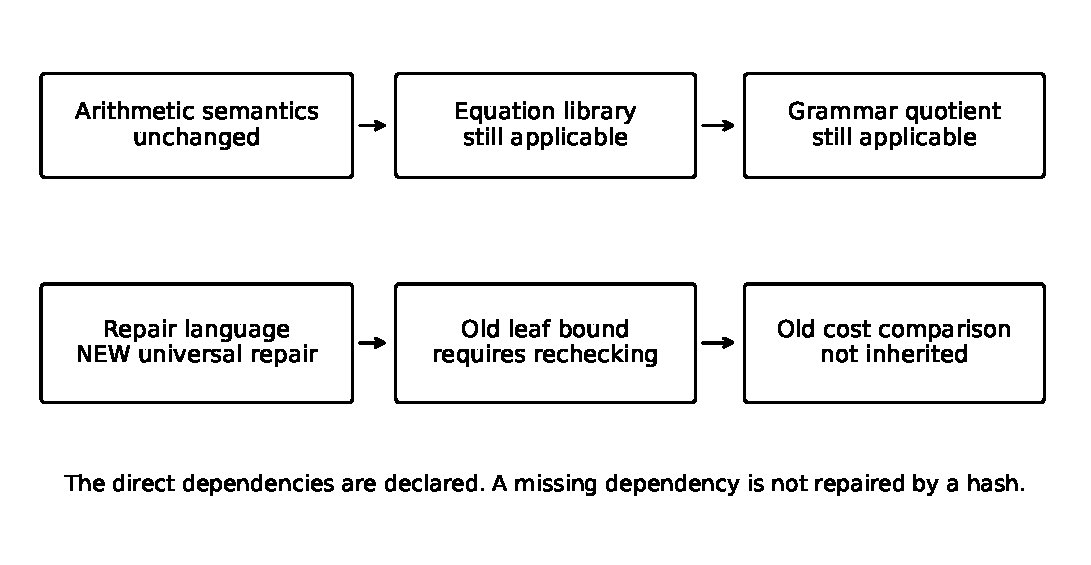
\includegraphics[width=\linewidth]{figures/revision_scope.pdf}
\caption{A change to the repair language affects the diagnostic justification but need not change arithmetic semantics. The depicted graph is a declared example, not an automatically discovered dependency registry.}
\end{figure}

\section{Semantic improvement and resource improvement are separate}
Fix named additive event types. Let $K\ge0$ be an extra preparation vector, let $s_i$ be the old-minus-new per-use vector for workload type $i$, and let $n_i$ count its uses. The net event difference is
\[
\Delta=\sum_i n_i s_i-K.
\]
A nonnegative price vector $w$ converts these events into one declared additive measure. Storage capacity, peak memory, and elapsed time need their own models unless a justified conversion is specified.

\begin{proposition}[Which gains survive every admitted price?]\label{r:prices}
The saving $w\cdot\Delta$ is nonnegative for every nonnegative price vector if and only if every coordinate of $\Delta$ is nonnegative. If prices lie in the convex hull of a finite nonempty set $W$, their minimum saving equals $\min_{w\in W}w\cdot\Delta$.
\end{proposition}
\begin{proof}
A componentwise nonnegative vector has nonnegative inner product with every nonnegative vector. If coordinate $j$ is negative, assigning price one only to that coordinate gives a negative result. This proves the first assertion. A point in the stated convex hull is a convex combination of its listed prices, so its saving is the same convex combination of their savings. It cannot be smaller than the minimum listed value, and a listed minimizer attains that value.
\end{proof}
\source{[SII], Proposition 25.1. No hardware performance law follows from this additive accounting identity.}

For the source's checked weighted-search comparison, the event difference is $(1552,1552,-1868)$ in reads, rational additions, and comparisons. Equal prices give $1236$ saved units. Prices $(1,0,1)$ give a loss of $316$. Both conclusions concern the same valid controller. The main text uses this as a transparently rechecked source calculation, not as a new measured timing result.

\section{Evidence across an adaptive sequence}
A procedure that searches many candidates can select a favorable error in its evaluator. The right statement must therefore condition on the information that produced the candidate, not merely repeat a marginal error bound for a candidate fixed in advance.

\begin{proposition}[A conditional error budget for a lineage]\label{r:lineage}
Let $\mathcal H_{j-1}$ contain the information available before attempt $j$. Suppose the event $A_j$ of accepting a false claim satisfies
\[
\Pr(A_j\mid\mathcal H_{j-1})\le\delta_j\quad\text{almost surely},
\qquad\sum_{j\ge1}\delta_j\le\delta,
\]
for deterministic nonnegative $\delta_j$. Then the probability of ever accepting any false claim is at most $\delta$, even when candidates and the stopping time depend on earlier history.
\end{proposition}
\begin{proof}
Taking expectations gives $\Pr(A_j)\le\delta_j$. A union bound gives the result for every finite set of attempts. The finite unions increase to the event of any false acceptance, so continuity of probability gives the infinite statement. Stopping removes attempted events and cannot enlarge their union.
\end{proof}
\source{[SII], Proposition 26.1. The mathematical input is conditional validity of each actual attempt. A numerical error schedule alone does not establish that premise.}

This proposition is not an empirical result about a population of agents. It explains what evidence would need to remain valid when an evaluator is used adaptively. Deterministic exact checks in this book are not treated as statistical samples and are not assigned confidence intervals through this formula.

\section*{What is now available}
A revision can preserve its meaning, identify stale obligations, and state its resource advantage under explicit prices. None of this yet determines what several participants can know together or which authority they should exercise. The next chapter keeps information sharing and institutional permissions separate while applying the same preservation discipline.

\chapter{Shared work and maintained obligations}\label{ch:shared}
\question{Joint information can support a task without creating a single decision maker.}
One agent may have a display record and another a calibration record. Neither need know the physical target bit alone. Together their records can determine it. This is an informational relation before it is any claim about collective agency.

\section{What several accessible records can reconstruct}
Let $V$ be a finite-dimensional vector space over a field. Participant $i$ has a linear record $A_i v$. Stack the records into $Av=(A_1v,\ldots,A_mv)$, and let $Qv$ be the protected linear target.

\begin{proposition}[Target-relative joint reconstruction]\label{r:reconstruction}
There is a linear decoder $D$ with $Q=DA$ if and only if $\ker A\subseteq\ker Q$. Full-state reconstruction is possible exactly when $A$ is injective. The intersection identity $\ker A=\bigcap_i\ker A_i$ determines which ambiguities sharing removes.
\end{proposition}
\begin{proof}
If $Q=DA$, a vector annihilated by $A$ is also annihilated by $Q$. Conversely, define $D(Av)=Qv$ on $\im A$. If $Av=Aw$, then $v-w\in\ker A\subseteq\ker Q$, so this definition is independent of the representative. It is linear and extends to the full record space by extending a basis. For $Q=I_V$ the kernel condition is injectivity. A stacked record vanishes exactly when each component record vanishes, giving the intersection identity.
\end{proof}
\source{Target-relative specialization of the reconstruction and factorization machinery in Sufficient Resolution [SR] and Stratified Relational Workspace Theory [SRWT]. The proof here does not import their complete noise, dynamics, or identity theories.}

Over $\mathbb F_2$, Agent A observes $A_A(b,s)=b+s$ and Agent B observes $A_B(b,s)=s$. The joint matrix is invertible. Either agent alone lacks a direction needed to recover $b$. The nuisance bit may remain unknown because the target map ignores it.

The theorem concerns accessible records. It does not send them. A communication protocol, truthful interpretation, permitted disclosure, and the recipient's executable decoder remain separate requirements. Chapter~\ref{ch:decision} states the corresponding fixed-recipient criterion.

\section{Permissions are part of an operational state}
Now let a finite institutional state $x$ have a protected label $\ell(x)$, an enabled-action set $D(x)$ within a fixed finite alphabet, and a deterministic successor $F(x,a)$ for enabled actions. Labels may include resource balances, outstanding obligations, and offices, but need not retain every historical byte.

\begin{theorem}[A quotient that preserves legal operations]\label{r:governance}
For a surjection $\pi:X\to Z$, quotient labels, enabled sets, and successors satisfying
\[
\ell=\bar\ell\pi,\qquad D=\bar D\pi,\qquad
\pi F(x,a)=\bar F(\pi x,a)
\]
exist exactly when equal fibres have equal labels, equal enabled sets, and equal projected successors for every enabled action. The quotient labels, enabled sets, and successors on enabled actions are unique. They preserve every legal finite action and label sequence. Values assigned by a totalized implementation to disabled actions are outside this uniqueness statement.
\end{theorem}
\begin{proof}
Factoring each quantity proves necessity. For sufficiency choose a representative of each fibre to define its label, enabled set, and successor. The three equalities make those definitions independent of the representative. Surjectivity gives uniqueness. Equal enabled sets admit the same first action, and successor equality preserves membership in one fibre. Induction on the sequence length preserves legality and all labels.
\end{proof}
\source{[MS], ``Exact governance quotient.'' This extends the deterministic behavioral construction by explicitly protecting action availability. It does not derive moral or external legal authority from the state description.}

A summary that preserves only the next sensor response can merge states in which a repair is authorized with states in which it is forbidden. It may remain a good predictor while becoming an invalid action interface. The necessary correction is to preserve the enabled-set distinction, not merely to attach a reassuring name to the old code.

\section{Continuing should not erase the ability to finish}
Use a finite \emph{observed} configuration space $Z$. Under partial observation, the configurations would instead have to be justified public possibility states. At $z$ there are finite catalogues of running actions and ending actions, each with a nonempty successor set. A declared safe set is $S$, and an ending target is $G\subseteq S$. A safe hold action is available at $G$.

A stop command is assumed authentic and observable before the next action is selected. Its delivery and authentication are premises, not consequences of the following fixed-point calculation. Define
\begin{align*}
T_0&=G,\\
T_{k+1}&=T_k\cup\{z\in S:\exists a\in A_{\rm end}(z),\ \operatorname{Post}(z,a)\subseteq T_k\}.
\end{align*}
Let $T_*$ be the stable set. Then define
\[
L_0=T_*,\qquad
L_{k+1}=\{z\in L_k:\exists a\in A_{\rm run}(z),\ \operatorname{Post}(z,a)\subseteq L_k\},
\]
and let $L_*$ be its stable value. Both sequences stabilize because $Z$ is finite.

\begin{theorem}[Safe continuation that retains an ending strategy]\label{r:ending}
A starting configuration belongs to $L_*$ exactly when one policy can run safely indefinitely without a stop command and, after a stop command at any decision epoch, reach $G$ on every possible successor path using only the admitted ending actions. Before the command a policy preserving $L_*$ suffices. After the command it can reach $G$ within the first-entry rank of the current state in the $T_k$ sequence.
\end{theorem}
\begin{proof}
Induction shows that membership in $T_k$ is equivalent to an ending-only policy reaching $G$ within $k$ transitions while staying safe. The chosen action moves every successor to a smaller rank. Outside $T_*$, every ending action has a successor outside $T_*$ or outside safety. Choosing such a successor at every step defeats any purported surely safe ending. Thus $T_*$ is exactly the sure-ending region.

At $L_*$ a running action keeps every successor inside $L_*$. Repeatedly using such actions is safe and retains membership in $T_*$. A command can therefore switch to the decreasing-rank ending policy at any epoch.

Conversely, if a policy has the stated guarantee, every pre-command reachable configuration must admit an ending immediately and hence lie in $T_*$. For any finite number of further running steps, it must keep all paths in that set. Induction in the decreasing construction places the initial state in every $L_k$, hence in $L_*$. No action is chosen after secretly observing its successor.
\end{proof}
\source{Fully observed finite specialization of [MS], ``Continued operation with an available authorized ending.'' The more general public-possibility construction is not silently assumed in this version.}

\begin{counterexample}[Safe inactivity without an ending]\label{ce:ending}
A state $z$ has a safe idle self-loop and no ending action reaching $G$. It is safe forever but outside $T_*$. In a second state $u$, an ending is available, while the only running action spends its reserved resource and moves to $z$. Then $u$ belongs to $T_*$ but not $L_*$. Being able to stop now does not establish that ordinary operation preserves that ability.
\end{counterexample}

These results do not establish society formation, strategic compliance, or a just constitution. They establish information, action, and continuation properties of a specified finite institution. Their place in this finite reasoning chain follows from the preceding account of accessible evidence, common artifacts, feasible controllers, and dependency-preserving revision.

\chapter{One continuous chain, with no hidden promotion}\label{ch:close}
The sensor story can now be followed without changing the meaning of a record midway through the argument.

Begin with eight candidate worlds $(b,s,n)$. The agent's initial display $y$ determines its two-state predictive class under flips, but not the physical target bit. The first chapter proves both claims. The second gives the operator on the retained class and the coordinate map that becomes usable after calibration. Neither requires the nuisance bit.

When display and calibration observations arrive, candidate sets are filtered. The third chapter proves why the joint association must be retained, and why sixteen occupancy states suffice for the exact partition-evidence contract. Under a separately declared noisy calibration, four probability masses replace the occupancy bits. The same numerical posterior cannot be inferred from separate marginals. The correction argument requires a joint report/next-state law, not only correct separate marginals. Its finite refinement makes the required distinctions explicit, and its history bound states the separate price of conditioning on a rare report.

The fourth chapter places that posterior and any response approximation under one loss function. It also specifies what a recipient can decode from a message and its prior record. The fifth asks whether the sender can acquire the missing observation and transmit a successful artifact within a single online and stored-controller budget. The complete tree is counted even if an execution visits only one path. A separate noisy-calibration calculation then uses the exact same retained belief to select a finite expected-cost inquiry. Uniform whole-history error supports a quantitative policy comparison, but not an automatic hard-budget or zero-risk guarantee.

The sixth chapter then changes the discovery procedure rather than the hidden world. Checked equations can remove equivalent candidates while preserving every teacher proposal and counterexample. A separately justified capacity rule can stop reading an impossible diagnostic root. Neither step invents the primitive grammar, the teacher, or the theorem used to authorize pruning.

The seventh chapter binds those uses to their premises. Adding a universal repair changes the required diagnostic distinctions. The old lower bound becomes inapplicable. Arithmetic identities can remain applicable. A fresh cost comparison may find a saving or a loss. The eighth chapter finally combines different participants' records and asks what actions they are entitled to perform under their declared institutional state. Safe indefinite operation and preservation of an authorized ending are checked separately.

\section{A worked end-to-end record}
Take the actual illustrative world $(b,s,n)=(0,1,1)$. The complete protocol begins with all eight worlds possible:
\begin{center}\begin{tabular}{p{0.25\linewidth}p{0.27\linewidth}p{0.35\linewidth}}\toprule
Event & Remaining worlds & What is justified\\\midrule
Before observation & All eight & No physical target identified.\\
Display $y=1$ & Four worlds & Predict every later display flip.\\
Calibration $s=1$ & Two worlds differing only in $n$ & Physical target $b=0$.\\
Send $y$ to a recipient holding $s$ & Same two worlds & Recipient computes $b=0$ through its fixed XOR decoder.\\
Commit the authorized target action & As declared by its effect & One action justified across the current support.\\
Record the fulfilled obligation & Includes the action's receipt & Continuation or ending can refer to the actual completed act.\\\bottomrule\end{tabular}\end{center}

The witness does not claim to have discovered its sensor semantics. Its exact checking confirms the stated scenario. Another physical process requires its own evidence. A failed receipt, an untrusted calibration, or an altered action effect changes the guarantee rather than being averaged away as a small numerical error.

\section{Why the core is narrower than the archive}
This book does not append the old Neuralese experimental history, proposed PRISM architecture, full SRIC lineage, or every formal guide. Their presence would make the reader repeatedly switch between a proved conditional statement, a proposed mechanism, a historical execution, and an implementation plan. Those are useful source objects, but they are not one continuous proof.

Selected source results are restated and proved where they carry the argument. Selected stochastic-value arguments from AVOC enter through complete proofs and explicitly matched finite models. Several resulting statements have source-facing counterparts in the archived Machine Theory development. The full AVOC implementation and the specialist Certified Bayesian Inference construction remain outside this selection. The correspondence appendix records the difference between those archived counterparts and the present editorial work.

Nor is a source excluded merely because it contains open questions. Its proved results can be considered individually. A claim enters when its exact form, dependencies, and evidence have been reviewed at the level promised for this edition. This is a stricter and more useful rule than treating every page of a final-named document as equally checked.

\section{The result of the compilation}
The core establishes a connected conditional account of accessible state, meaningful operations, corrective memory, usable explanations, bounded investigations, justified search changes, and maintained obligations. The arguments share several elementary constructions, but each use preserves its distinct type and hypotheses.

No theorem here turns a semantic interface into a trained neural model, a finite investigation into general intelligence, a shared record into a collective subject, or an invariant into legitimate external authority. The mathematical contribution is the explicit chain and the failures that break it. Those failures can be investigated without changing the standard of proof or requiring a large implementation campaign.


\part{Composition, control, and revision}
\chapter{A common contract for stochastic and legal operations}\label{ch:jointcontract}

A probability model describes what an action may do. An action catalogue describes whether that action is available. A useful abstraction may need to preserve both. Keeping a correct next-state marginal while losing the report correlation can destroy a filter. Keeping the correct filter while losing a permission distinction can admit an action that the underlying model forbids.

The two preservation problems use one state map in this chapter. Their composition is exact for a supplied finite model. The proof also specifies what the policy can observe, because a comparison between two models is meaningless if their controllers secretly receive different information.

\section{The joint data of a decision process}
Let $X$ and $Z$ be finite nonempty state sets and let $\pi:X\to Z$ be surjective. Let $A$ and $O$ be finite nonempty action and report alphabets. At a fine state $x$, the set $D(x)\subseteq A$ contains the admitted actions, and $\ell(x)\in Y$ is a protected label. For $a\in D(x)$, the nonnegative numbers
\[
 K_{a,o}(x'\mid x),\qquad
 \sum_{o\in O}\sum_{x'\in X}K_{a,o}(x'\mid x)=1
\]
specify the joint distribution of the next state and report. No transition is specified for a disabled action. An implementation may fill unused entries, but those values have no role in the contract.

For a nonnegative vector $u$ on $X$, write
\[
 (\pi_*u)(z)=\sum_{\pi x=z}u(x).
\]
This notation applies to probability distributions and to unnormalized history masses. A coarse model has labels $\bar\ell$, enabled sets $\bar D$, and joint instruments $\bar K$ on its enabled actions.

\begin{theorem}[Joint legal and stochastic quotient criterion]\label{r:joint-quotient}
There are coarse data satisfying
\[
 D(x)=\bar D(\pi x),\quad \ell(x)=\bar\ell(\pi x),\quad
 \sum_{\pi x'=z'}K_{a,o}(x'\mid x)=\bar K_{a,o}(z'\mid\pi x)
\]
for every $x$, every $a\in D(x)$, and every $o,z'$, if and only if states in the same fibre have identical labels and enabled sets and identical projected joint successor/report rows. Explicitly, $\pi x=\pi y$ must imply
\begin{align}
 D(x)&=D(y),\qquad \ell(x)=\ell(y),\label{eq:fibre-legal}\\
 \sum_{\pi x'=z'}K_{a,o}(x'\mid x)
 &=\sum_{\pi x'=z'}K_{a,o}(x'\mid y)
 \quad(a\in D(x),\ o\in O,\ z'\in Z).\label{eq:fibre-joint}
\end{align}
When these conditions hold, the coarse labels, enabled sets, and instruments on enabled actions are unique.
\end{theorem}
\begin{proof}
The factorization identities give necessity immediately. For sufficiency, choose a representative $x$ of each fibre. Define its coarse label and enabled set by their values at $x$, and define the coarse instrument by the displayed fibre sum. The hypotheses make all three choices independent of the representative. The new entries are nonnegative. Summing them over $o,z'$ sums every fine successor exactly once and therefore gives one. Surjectivity gives uniqueness at every coarse state. Uniqueness says nothing about padded values for disabled actions.
\end{proof}

\section{Observable histories and common admissibility}
A history available to the policy is
\[
 h=(a_1,o_1,\ldots,a_t,o_t).
\]
The fine hidden state and the coarse state are not additional policy inputs. Protected labels are recorded for comparison, but are not assumed observed merely because the theorem preserves them. An application that exposes a label must include it in the observation interface of both models.

Start from a fine prior $p_0$ and the coarse prior $\bar p_0=\pi_*p_0$. Let $u_h(x)$ be the unnormalized probability of history $h$ and current state $x$. A common policy assigns the same probability $\alpha(a\mid h)$ in both models. At every positive-mass history it may select only actions in
\[
 D_h=\bigcap_{x:u_h(x)>0}D(x).
\]
The intersection is over a nonempty support. If it is empty, no policy can make another admitted action at that history. A stopping convention can be included as a shared terminal action, but is not silently supplied by a stochastic row.

\begin{lemma}[Support and admissible actions agree]\label{r:joint-support}
If $\bar u_h=\pi_*u_h$, then
\[
 \operatorname{supp}\bar u_h=\pi(\operatorname{supp}u_h),\qquad
 \bigcap_{x:u_h(x)>0}D(x)=\bigcap_{z:\bar u_h(z)>0}\bar D(z)
\]
whenever the history has positive mass.
\end{lemma}
\begin{proof}
A finite sum of nonnegative terms is positive exactly when at least one summand is positive. This gives the support identity. The enabled sets are constant on each fibre, so repeating a fibre's action set in an intersection changes nothing. The two intersections are therefore equal.
\end{proof}

\begin{theorem}[Preservation of complete controlled histories]\label{r:joint-history}
Under Theorem~\ref{r:joint-quotient}, a common admissible history policy preserves the law of every finite coarse-state/action/report path. Consequently it preserves every action/report/label history. At every positive-mass history it also preserves the aggregated posterior and the set of actions admitted throughout its support. These claims hold at every horizon for which the policy is defined on all positive-mass prefixes.
\end{theorem}
\begin{proof}
First prove $\bar u_h=\pi_*u_h$ by induction. It holds initially by the prior assumption. At a positive history, Lemma~\ref{r:joint-support} gives the same available actions on both sides. For any action with positive policy mass, every current fine state of positive mass enables that action. Thus
\[
 \pi_*u_{hao}
 =\pi_*\bigl(\alpha(a\mid h)K_{a,o}u_h\bigr)
 =\alpha(a\mid h)\bar K_{a,o}\pi_*u_h
 =\bar u_{hao}.
\]
Here multiplication uses only enabled columns. Values in all other columns are irrelevant because their input mass is zero. Zero-mass prefixes stay zero. Summation proves equality of history probabilities, and division by the common positive mass proves the posterior assertion.

This induction alone records only the current state and the observed history. To retain the entire state path, fix a coarse prefix
\[
 (z_0,a_1,o_1,z_1,\ldots,a_t,o_t,z_t).
\]
Sum fine path weights over all fine prefixes mapping to this prefix. For one more step, each fine current state in the last fibre contributes the same projected successor/report row by Equation~\eqref{eq:fibre-joint}. The policy factor depends only on the already fixed action/report prefix. It can therefore be taken outside the fine-state sum. Induction gives the exact path mass
\[
 \bar p_0(z_0)\prod_{i=1}^{t}
 \alpha(a_i\mid a_1,o_1,\ldots,a_{i-1},o_{i-1})
 \bar K_{a_i,o_i}(z_i\mid z_{i-1}).
\]
An inadmissible or zero-mass prefix contributes zero. This is precisely the coarse path law. Applying $\bar\ell$ to each $z_i$ gives the full label history, including its correlations across time. Labels need not be disclosed to the policy for this pushforward comparison to be valid.
\end{proof}

\source{This is a joint finite composition of Theorems~\ref{r:instrument} and~\ref{r:governance}. The path argument and the common-support lemma are explicit parts of the present statement. The result is a written proof, not a newly compiled Lean theorem.}

\section{Why preserving two marginals is insufficient}
Consider two fine states in one proposed coarse input fibre. From the first, the pairs $(z',o)$ are $(0,0)$ and $(1,1)$ with probability $1/2$ each. From the second, they are $(0,1)$ and $(1,0)$ with probability $1/2$ each. The successor marginal and the report marginal are both uniform in either case. Their association is different, however, so the same report leads to opposite posterior states. Equation~\eqref{eq:fibre-joint} fails.
\begin{figure}[htbp]\centering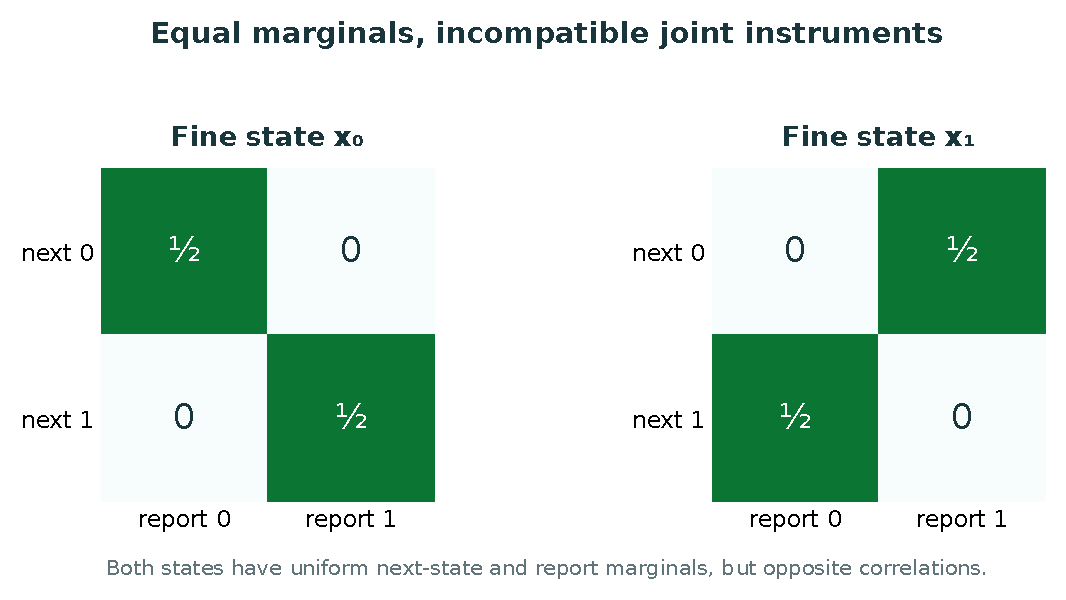
\includegraphics[width=.87\linewidth]{figures/joint_instrument_obstruction.pdf}\caption{Equal marginals do not determine the joint instrument. Each table is an exact probability law. The report needed for correction is correlated with opposite successor states.}\label{fig:joint-obstruction}\end{figure}

Final-state checks have a different limitation. Two deterministic paths can visit different intermediate labels and return to the same final state. A test that stores only the terminal state and the report word cannot distinguish them when the reports omit those labels. Complete path preservation requires the prefix argument above, not just a terminal distribution comparison.

\section{An exact sensor realization}
Return to $x=(b,s,n)\in\{0,1\}^3$ and retain $z=(b,s)$. The actions \emph{hold} and \emph{flip} are available everywhere. A \emph{repair} action is available only where $b=0$ and leaves that target value fixed. The nuisance bit is retained by every fine transition but ignored by the coarse state.

After an action, report the new display $b\oplus s$ correctly with probability $3/4$ and incorrectly with probability $1/4$. Both the label and the joint instrument ignore $n$. The ten coarse state/action rows satisfy the quotient conditions exactly.

From a uniform prior, a report leaves both target values possible, so repair is not uniformly admitted. A policy that reacts to those reports must continue with hold or flip. From a prior supported on $b=0$, repair is available until an action changes that support. The distinction exercises the support condition rather than assuming all actions are always available.

The reference checker compares complete projected state paths, action words, report words, and label words under deterministic and randomized report policies. It also compares every positive-history posterior and available-action intersection. The exact finite examples supplement the general proof. Their probabilities and action semantics are supplied model data.

\section{Three different failures}
A quotient may lose a protected label or an enabled-action distinction. It may preserve separate probability marginals and lose their joint law. Or it may be mathematically exact but unavailable to a learner whose evidence cannot initialize it. The first two are failures of preservation. The third is a failure of acquisition. A correction must address the failed condition rather than merely increase the size of the retained vector.

\chapter{Preserving an ending strategy under safe continuation}\label{ch:endinganalysis}

A system may remain within a declared safe region indefinitely and still lose every way to end its operation. Conversely, an authorized ending procedure may exist at the present state but become unavailable after the next ordinary action. These are distinct requirements. The relevant mathematical object is therefore not a safety invariant alone, but a safe-running region entirely contained in a sure-ending region.

The following development expands the finite result stated earlier in Chapter~\ref{ch:shared}. It supplies an explicit rank proof, treats strategies that depend on observed history, and separates deadlock from an infinite unsuccessful path. Formal correspondence is recorded in the appendix.

\section{Finite game data and the command boundary}
Fix a finite, fully observed configuration set $Z$. Each $z\in Z$ has finite collections $A_{\rm run}(z)$ of running actions and $A_{\rm end}(z)$ of ending actions. For each admitted action $a$ there is a nonempty set $\operatorname{Post}(z,a)\subseteq Z$ of possible successors. A controller chooses an action \emph{before} the successor is determined. The quantifier over all successors is adversarial and is stronger than an expected-value objective.

Let $S\subseteq Z$ be a safe set and $G\subseteq S$ an ending target. At every state of $G$, a hold operation with successors contained in $G$ is available after ending. Running forever means that the controller can choose an admitted action at every pre-command epoch. Deadlock is not counted as successful indefinite operation. A stop command is authenticated and observed before the next action is selected. Whether such an authentication protocol exists in an external institution is not proved by the game calculation. It is part of the model supplied to this theorem.

A strategy may inspect the finite history of observed states and chosen actions. Before the stop command it selects running actions. After the command it selects ending actions. The desired guarantee consists of two clauses: every running path without a command remains safe forever, and every path following a command at any decision epoch reaches $G$ in finitely many ending steps while remaining safe. The strategy must satisfy both clauses under the same command-conditioned policy.

\section{The sure-ending attractor}
Define
\begin{align*}
T_0&=G,\\
T_{k+1}&=T_k\cup\left\{z\in S:\text{some }a\in A_{\rm end}(z)
\text{ satisfies }\operatorname{Post}(z,a)\subseteq T_k\right\}.
\end{align*}
The sequence is increasing and every term is contained in $S$. Because the state set is finite, it becomes constant after finitely many strict additions. Let $T_*$ denote its stable value. For $z\in T_*$, define the first-entry rank $\rho(z)$ as the least $k$ with $z\in T_k$.

\begin{lemma}[Finite-horizon ending criterion]\label{r:end-horizon}
A configuration $z$ belongs to $T_k$ exactly when there exists an ending-only strategy that, whatever the successors, reaches $G$ within at most $k$ transitions while remaining in $S$. In particular, if $\rho(z)>0$, there is an ending action whose every successor has strictly smaller first-entry rank.
\end{lemma}
\begin{proof}
The assertion at $k=0$ says precisely that the initial state is already in $G$. Assume it holds for $k$. If $z\in T_{k+1}\setminus T_k$, the construction supplies an ending action with all successors in $T_k$. After the action the controller uses the strategy given by induction for the observed successor. Every path reaches $G$ within another $k$ transitions. States already in $T_k$ retain their strategy. Conversely, a policy that reaches $G$ in at most $k+1$ steps must either start in $G$, or select some first ending action such that the continuation from every possible successor reaches $G$ within $k$ steps. By induction every such successor belongs to $T_k$, hence the initial state lies in $T_{k+1}$. At the first-entry stage $\rho(z)$, the selected action sends every successor into $T_{\rho(z)-1}$, establishing strict rank decrease.
\end{proof}

\begin{lemma}[Adversarial completeness of the ending region]\label{r:ending-complete}
From a configuration outside $T_*$, no strategy, including one depending on arbitrary finite observed history, can guarantee safe eventual arrival at $G$ along every successor path.
\end{lemma}
\begin{proof}
If the initial configuration is outside $S$, safety has already failed. Otherwise, because $T_*$ is a fixed point, no ending action at a state $z\in S\setminus T_*$ can have all its successors in $T_*$. An adversary can therefore select a successor outside $T_*$ after every proposed ending action. If the selected successor is outside $S$, safety fails. If it remains within $S\setminus T_*$, the same argument can be repeated. The adversary does not need to know the controller's future choices, only its chosen action at each current state. If the controller reaches a non-goal state with no ending action, it deadlocks before reaching the target and loses. Otherwise, either safety fails at a finite step or an infinite path never reaches $G$, which is contained in $T_*$. This defeats any sure-ending guarantee. The argument permits history-dependent policies and requires nonempty successor sets so that the proposed actions represent actual transitions.
\end{proof}

These lemmas show that $T_*$ is not merely the region reached by a convenient algorithm. It is \emph{exactly} the set from which an ending strategy can guarantee success under all modeled successor choices. The rank bounds the required ending transitions by a finite number no greater than the number of strict expansion rounds.

\section{A safety invariant that retains the ending region}
The ending region is not necessarily closed under ordinary running. Define the decreasing sequence
\[
L_0=T_*,\qquad
L_{k+1}=\left\{z\in L_k:\exists a\in A_{\rm run}(z),\ \operatorname{Post}(z,a)\subseteq L_k\right\}.
\]
Let $L_*$ be its stable value. Each stage removes states for which ordinary operation cannot be guaranteed to remain in the preceding stage.

\begin{lemma}[Greatest controlled invariant inside the ending region]\label{r:running-invariant}
The set $L_*$ is the greatest subset of $T_*$ admitting a running action at every member with all successors again in that subset. A state belongs to $L_k$ exactly when a strategy can safely take $k$ running actions while leaving a sure-ending strategy available at every reached decision epoch, including the initial one.
\end{lemma}
\begin{proof}
The bounded-horizon claim follows by induction. At horizon zero only membership in $T_*$ is needed. For the next step, a first running action must send every successor to a state that permits the remaining $k$ running steps and an ending option at every intermediate epoch. Truncating a successful $(k+1)$-step strategy after $k$ steps also shows that its initial state lies in $L_k$. Thus the initial state and all successors of its first action lie in $L_k$, exactly as required by $L_{k+1}$. Conversely, membership supplies the first action and the inductive strategies from its successors.

At stabilization, the defining equation gives one running action for each state in $L_*$ whose successors stay in $L_*$. Selecting these actions proves controlled invariance. If $B\subseteq T_*$ is any other subset with the same property, induction shows $B\subseteq L_k$ for every $k$: inclusion at zero is given. The witnessing running action for any $z\in B$ has all successors in $B\subseteq L_k$, so $z\in L_{k+1}$. Thus $B\subseteq L_*$. No larger controlled invariant within $T_*$ exists.
\end{proof}

\begin{theorem}[Safe running with an available ending at every epoch]\label{r:joint-ending}
A state $z$ belongs to $L_*$ if and only if a single command-conditioned policy can run safely forever in the absence of a command and, upon receiving an authentic stop command at any decision epoch, can reach $G$ on every possible successor path using only ending actions. The stopping phase from a state $w$ reaches $G$ within $\rho(w)$ transitions. The combined policy can be chosen positional in the pair consisting of the current state and the command mode.
\end{theorem}
\begin{proof}
For sufficiency, at each running state in $L_*$ choose an action with all successors in $L_*$. Such actions exist by the preceding lemma and keep every running path within $L_*\subseteq T_*\subseteq S$ for any duration. If a stop command arrives at a decision epoch, the current state still lies in $T_*$. Switch modes and choose a first-entry-rank-decreasing ending action. The rank is a nonnegative integer, decreases strictly after every ending transition outside $G$, and must reach zero in no more than $\rho(w)$ steps. At rank zero the system is in $G$ and can hold safely. This is one policy with the command as its observable mode switch, not two incompatible policies chosen after seeing a future path.

For necessity, consider any policy with the stated guarantee, including one that depends on the entire available history. The stop command may arrive at the present epoch, so by the adversarial completeness lemma the starting state must belong to $T_*$. It may instead arrive after any number $k$ of running steps. Every state reachable immediately before such a command must therefore remain in $T_*$. The running prefix of length $k$ consequently satisfies the bounded-horizon condition of the preceding lemma, so the initial state is in $L_k$. This holds for every $k$. The decreasing sequence stabilizes on a finite set, hence the state belongs to its eventual value $L_*$. No operation is selected with advance knowledge of which successor an adversary will return.
\end{proof}

\section{A three-state obstruction to naive safety}
Consider the safe configurations $S=\{u,z,g\}$ with ending target $G=\{g\}$. The state $g$ has a hold action in both modes, $z$ has a safe running self-loop but cannot end, and $u$ can end immediately at $g$. Yet the only running action at $u$ moves to $z$. This gives
\[
T_*=\{u,g\},\qquad L_*=\{g\}.
\]
It is possible to end from $u$ now, but not to run from $u$ while retaining the option to end later. The obstruction is about \emph{future control access}, not immediate safety.
\begin{figure}[htbp]\centering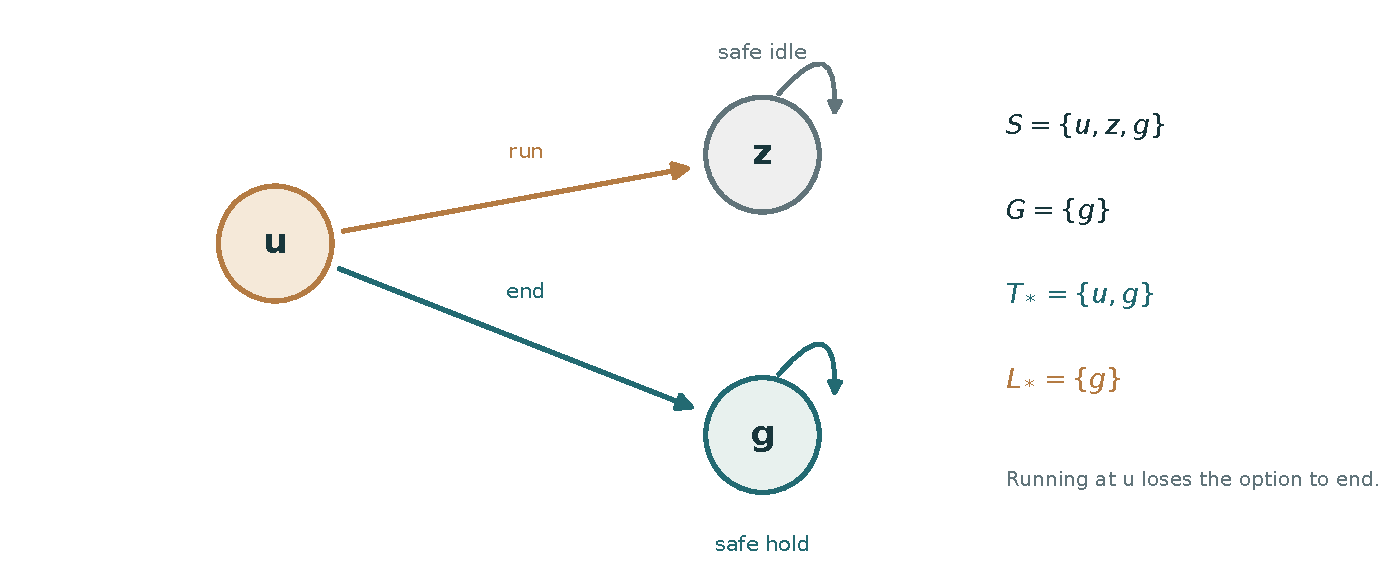
\includegraphics[width=.95\linewidth]{figures/safe_ending_kernel.pdf}\caption{Exact finite safe-running and sure-ending example. The initial running action from $u$ loses the ending option. The sets were checked against explicit strategy enumeration.}\label{fig:ending-kernel}\end{figure}

The companion verifier compares the fixed-point calculation with explicit positional-policy enumeration and checks the rank-decreasing witnesses. The exact input domains and results appear in the verification guide. The calculation treats arrival at $G$ as termination. The stipulated hold concerns subsequent behavior and does not change the reachability calculation.

\section{What changes with partial observation}
The proof assumes the actual configuration is observed when an action is chosen. If only a public report is available, strategies generally act on a belief or possibility state whose update must be justified by the observation protocol. Replacing $Z$ with arbitrary hidden-state names does not produce a valid partially observed ending theorem. One would need a common public-state construction, exact reporting and successor semantics, and a proof that the stop command is observed before action selection. The finite theorem is a solid component of that larger problem without silently solving it.

\chapter{Transporting safe continuation through a quotient}\label{ch:controltransport}

The previous chapters establish a stochastic quotient and a safe-ending game separately. To use both in one system, the retained state must also preserve the successor choices relevant to a sure guarantee. Probabilities and supports have different roles here. A small positive transition probability still creates a possible path. It cannot be discarded in a claim that quantifies over every path.

This chapter gives an exact interface between representation change and the two fixed-point constructions. It then weakens equality to a one-sided enclosure that can certify an entire family of models.

\section{The controlled predecessor}
Let $X,Z$ be finite nonempty sets and $\pi:X\to Z$ a surjection. Use a common finite action alphabet with separate running and ending catalogues $A^X_m(x)$ and $A^Z_m(z)$, where $m\in\{\mathrm{run},\mathrm{end}\}$. Every admitted action has a nonempty successor set. The mode can be included in the action name, so the same printed action in two modes need not denote the same transition.

Assume the fine and coarse safe and goal sets agree by inverse image:
\[
 S_X=\pi^{-1}(S_Z),\qquad G_X=\pi^{-1}(G_Z),\qquad G_Z\subseteq S_Z.
\]
This is a substantive restriction. A label that distinguishes a safe state from an unsafe state cannot be omitted from a safety-preserving quotient.

For $B\subseteq X$, define the mode-specific predecessor
\[
 \operatorname{CPre}^X_m(B)
 =\{x:\exists a\in A^X_m(x),\ \operatorname{Post}_X(x,a)\subseteq B\}.
\]
Define $\operatorname{CPre}^Z_m$ in the same way. These operators do not themselves include a safety test. Safety enters the ending recurrence through its intersection with $S$, and the running recurrence through its current set.

\begin{lemma}[Predecessors commute with an exact controlled quotient]\label{r:control-predecessor}
Suppose, for each mode and fine state,
\begin{align*}
 A^X_m(x)&=A^Z_m(\pi x),\\
 \pi(\operatorname{Post}_X(x,a))&=\operatorname{Post}_Z(\pi x,a)
 \qquad(a\in A^X_m(x)).
\end{align*}
Then for every $B\subseteq Z$,
\[
 \operatorname{CPre}^X_m(\pi^{-1}B)
 =\pi^{-1}(\operatorname{CPre}^Z_m(B)).
\]
\end{lemma}
\begin{proof}
For an admitted action,
\[
 \operatorname{Post}_X(x,a)\subseteq\pi^{-1}B
 \quad\Longleftrightarrow\quad
 \pi(\operatorname{Post}_X(x,a))\subseteq B.
\]
Replace the projected successor set by its assumed coarse value. The action ranges in the two existential quantifiers are identical, so existence of a witnessing action is equivalent on both sides.
\end{proof}

\section{Transport of both fixed-point sequences}
Construct $T^X_k,L^X_k$ on the fine game and $T^Z_k,L^Z_k$ on the coarse game as in Chapter~\ref{ch:endinganalysis}. In particular, the running sequence starts from the stable ending region in its own model.

\begin{theorem}[Ending regions, running kernels, and ranks are preserved]\label{r:control-transport}
Under the exact controlled-quotient assumptions,
\[
 T^X_k=\pi^{-1}(T^Z_k),\qquad
 T^X_*=\pi^{-1}(T^Z_*),\qquad
 L^X_k=\pi^{-1}(L^Z_k),\qquad
 L^X_*=\pi^{-1}(L^Z_*)
\]
for every finite $k$. For every $x\in T^X_*$, the first-entry ranks agree:
\[
 \rho_X(x)=\rho_Z(\pi x).
\]
A positional coarse policy for safe continuation and ending lifts to a fine policy with the same rank bound. To execute that lift, the controller needs the current coarse state and command mode, but not the remaining fine-state coordinates.
\end{theorem}
\begin{proof}
The goal-set assumption gives equality at $T_0$. Inverse images commute with union and intersection. Applying Lemma~\ref{r:control-predecessor} to the ending predecessor gives the induction step
\begin{align*}
 T^X_{k+1}
 &=T^X_k\cup\bigl(S_X\cap\operatorname{CPre}^X_{\rm end}(T^X_k)\bigr)\\
 &=\pi^{-1}\!\left(T^Z_k\cup
       (S_Z\cap\operatorname{CPre}^Z_{\rm end}(T^Z_k))\right).
\end{align*}
The finite increasing sequences stabilize, so their stable sets also agree by inverse image. The first stage at which $x$ appears is exactly the first stage at which $\pi x$ appears, proving rank equality.

The equality of stable ending sets gives the base of the running induction. The recurrence is intersection with the running predecessor. The same inverse-image calculation proves equality at every running stage and hence at stabilization.

At a coarse state in $L^Z_*$, choose a running action whose successors remain in that set. It is admitted at every fine representative, and all its fine successors lie in $\pi^{-1}(L^Z_*)=L^X_*$. After the command, choose a coarse ending action that decreases rank. Its projected successors have smaller coarse rank, so every fine successor has smaller fine rank. These choices define the lifted policy.
\end{proof}

The equality is stronger than soundness of one selected policy. A fine state is winning exactly when its coarse image is winning, even if a proposed fine policy uses additional hidden coordinates. Chapter~\ref{ch:endinganalysis} characterizes all winning states through the fixed points, including those achievable by history-dependent policies. An exact quotient therefore does not conceal a better sure-ending strategy that depends on discarded state.

This does not give the controller an observation it did not have. A report-only policy from Chapter~\ref{ch:jointcontract} need not know its current coarse state. Applying the policy-lifting conclusion requires that $\pi x$ be observed or reconstructed from an available record. Equality of the abstract winning regions alone does not solve a partially observed control problem.

\section{From stochastic rows to successor supports}
Suppose a mode's game successors are exactly the support of the stochastic instrument:
\[
 \operatorname{Post}_X(x,a)
 =\{x':\exists o,\ K_{a,o}(x'\mid x)>0\}.
\]
Define the coarse successor set from $\bar K$ in the same way.

\begin{corollary}[An exact stochastic quotient preserves the support game]\label{r:stochastic-support-game}
The joint quotient of Theorem~\ref{r:joint-quotient} gives
\[
 \pi(\operatorname{Post}_X(x,a))=\operatorname{Post}_Z(\pi x,a)
\]
for every enabled action. If the mode catalogues and the safe and goal sets satisfy the preceding compatibility conditions, Theorem~\ref{r:control-transport} applies to the resulting support games.
\end{corollary}
\begin{proof}
For each $o,z'$, the coarse entry is a finite sum of nonnegative fine entries. It is positive exactly when at least one fine successor in that fibre has a positive entry for that report. Taking the union over reports gives the support identity. Normalization makes the support of every enabled action nonempty. The remaining hypotheses are precisely those of Theorem~\ref{r:control-transport}.
\end{proof}

A sure guarantee in this support game covers all supported successor paths. It is stronger than almost-sure success under a probability law. An infinite path can have probability zero while every one of its finite prefixes has positive probability. The support-game interpretation deliberately retains that path.

\section{Conservative enclosures give one-sided certificates}
Exact equality is not needed to certify a policy conservatively. Suppose instead that a coarse envelope admits only actions available at every fine representative and includes all projected actual successors:
\[
 A^Z_m(\pi x)\subseteq A^X_m(x),\qquad
 \pi(\operatorname{Post}_X(x,a))
 \subseteq\operatorname{Post}_Z(\pi x,a)
 \quad(a\in A^Z_m(\pi x)).
\]
The envelope may contain additional adverse successors and may omit some fine actions. Retain the exact inverse-image assumptions for safety and goals.

\begin{proposition}[A winning envelope policy remains winning]\label{r:control-envelope}
Under these one-sided assumptions,
\[
 \pi^{-1}(T^Z_*)\subseteq T^X_*,\qquad
 \pi^{-1}(L^Z_*)\subseteq L^X_*.
\]
A coarse ending rank bounds the ending time of the lifted policy. The same coarse policy works for every fine model satisfying the enclosure assumptions. The reverse inclusions need not hold.
\end{proposition}
\begin{proof}
Induction on the coarse ending stages proves
$\pi^{-1}(T^Z_k)\subseteq T^X_k$. A witnessing coarse action is available at each fine representative. Its actual successors project into the envelope's successors and hence into the previous coarse stage. The fine action therefore witnesses the next fine stage. The same argument proves rank decrease along every lifted ending path.

The inverse image of $L^Z_*$ lies inside $T^X_*$ by the first inclusion. Choose the coarse invariant running action at each coarse state. Every fine successor lies in the inverse image of $L^Z_*$. Thus that inverse image is a controlled invariant subset of the fine ending region. The greatest-invariant characterization places it inside $L^X_*$. The argument uses only the enclosure relations and therefore applies to every model satisfying them.
\end{proof}

A conservative rejection is not a proof that the fine problem is impossible. For example, a coarse envelope may include an unsafe successor that the actual fine model never reaches. The envelope can then reject a state from which the actual model has an immediate safe ending. The conclusion is intentionally one-sided.

\section{Why a small probability error is not a sure guarantee}
Take three states $s,g,b$, with safe set $\{s,g\}$ and goal $\{g\}$. Running holds $s$ or $g$ in place. The nominal ending action at $s$ moves to $g$ with probability one. The perturbed action instead moves to $g$ with probability $1-\epsilon$ and to unsafe state $b$ with probability $\epsilon$, where $0<\epsilon<1$. A hold action is available at $g$.

The row total variation distance is exactly $\epsilon$. In the nominal game, $s$ belongs to both the ending region and the running kernel. In the perturbed support game, the only ending action from $s$ has an unsafe successor, so $s$ belongs to neither. This happens for every positive $\epsilon$, however small.

\begin{figure}[htbp]\centering
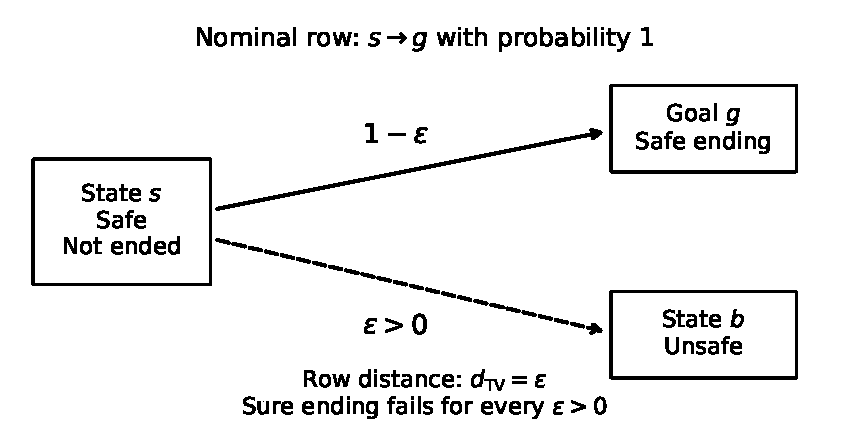
\includegraphics[width=.91\linewidth]{figures/support_margin.pdf}
\caption{An arbitrarily small unsafe branch changes a sure-ending certificate. The nominal and perturbed rows are exact declared distributions. Total variation controls probability discrepancy, not the disappearance of a supported adverse path.}\label{fig:support-margin}
\end{figure}

The appropriate robust certificate is an enclosure containing every possible successor, together with an action that succeeds throughout that enclosure. A small numerical residual is useful evidence for other purposes, but it cannot replace that quantified condition.

\section{The resulting integration}
We can now state the connection without changing the meaning of any interface. The stochastic quotient preserves controlled history laws. Its nonnegative rows induce an exact quotient of support games. Compatible safety and target labels then preserve the ending attractor, running kernel, and first-entry rank. Implementing the coarse policy still requires access to its current coarse state. Keeping these conditions separate is what makes the combined statement usable.

\chapter{Changing a representation without losing correctability}\label{ch:migration}

A representation can be sufficient for yesterday's questions and insufficient for today's. The old theorem need not be false. Its target may have changed. A revision procedure must therefore distinguish two tasks: translating information already retained and acquiring information that the old record discarded.

The simplest exact model makes this distinction precise. It also gives a constructive lower bound on the extra information required when a direct migration is impossible.

\section{A migration map exists exactly on constant fibres}
Let $H$ be a finite nonempty set of possible source histories. A history may include a model tag or a past observation whose value must remain available for later correction. Let
\[
 M:H\to U,\qquad N:H\to V
\]
be the old record and the required new record. Work on their attained images $U_0=M(H)$ and $V_0=N(H)$. The new record must be specified before sufficiency is claimed. It can be an answer, a correction signature, or the complete profile of future outputs in a declared finite contract.

\begin{theorem}[Exact migration criterion]\label{r:migration}
There is a map $J:U_0\to V_0$ satisfying $JM=N$ if and only if
\[
 M(h)=M(h')\quad\Longrightarrow\quad N(h)=N(h')
 \qquad(h,h'\in H).
\]
When it exists, $J$ is unique on attained old records.
\end{theorem}
\begin{proof}
Necessity follows by applying $J$ to the equal old records. Conversely, define $J(M(h))=N(h)$. The fibre condition makes the definition independent of the representative. Every $u\in U_0$ has such a representative, so the same equation determines $J$ uniquely.
\end{proof}

\source{This is the attained-record factorization of Proposition~\ref{r:factor}, applied to a representation revision. Grounded Abstraction [GA] supplies the correction-memory and evidence-migration setting. The argument does not assert a separate novelty claim for the fibre criterion.}

A collision with unequal new records is a complete obstruction to an exact deterministic migration from the old record alone. Adding more computation cannot distinguish the two histories. A randomized translator cannot be certainly correct on both either: the same old input gives the same output law, which cannot be concentrated at two different required values.

\section{What additional evidence must provide}
Suppose an allowed observation produces $E:H\to W$. A translator can use the pair $(M(h),E(h))$ rather than $M(h)$ alone.

\begin{corollary}[Evidence-assisted migration]\label{r:migration-evidence}
An exact translator from the available pair $(M,E)$ to $N$ exists if and only if
\[
 M(h)=M(h'),\ E(h)=E(h')\quad\Longrightarrow\quad N(h)=N(h').
\]
If a collision remains after the observation, that particular evidence interface cannot support the requested migration.
\end{corollary}
\begin{proof}
Apply Theorem~\ref{r:migration} to the record $h\mapsto(M(h),E(h))$.
\end{proof}

This result does not choose a physical observation or show that the observation is affordable. It tests the information supplied by a specified observation. A protocol with several actions can be treated similarly once its complete attained transcript is defined. Its admissibility, state changes, and costs then require the controller analysis of Chapter~\ref{ch:inquiry}.

\section{The least joint refinement}
When both the old and new uses must remain available, retain
\[
 P(h)=(M(h),N(h))\in P(H).
\]
The projections recover each record. No ordering between the old and new information is required.

\begin{proposition}[Universal property of the joint record]\label{r:joint-refinement-record}
If a record $R:H\to W$ determines both $M$ and $N$, then it determines $P$. In particular, $|R(H)|\ge |P(H)|$. The pair record attains this lower bound among records required to preserve both uses.
\end{proposition}
\begin{proof}
Let $fR=M$ and $gR=N$ on $H$. Then $w\mapsto(f(w),g(w))$ maps every attained value of $R$ to the corresponding attained pair. This map is onto $P(H)$, since every pair comes from a source history. Finiteness gives the cardinality inequality. The record $P$ itself has the required two projection maps.
\end{proof}

This is a statement about distinct attained values, not the byte size of a particular data structure. It allows the new state to discard duplicated encodings while preserving both information contracts.

\begin{theorem}[Minimum fixed-length supplementary information]\label{r:migration-bits}
For $u\in U_0$, put
\[
 k(u)=|N(M^{-1}\{u\})|,\qquad k_* =\max_{u\in U_0}k(u).
\]
Suppose an auxiliary encoder may inspect the complete source history and sends one fixed-length binary word in addition to the old record. Exact recovery of $N$ is possible with $b$ supplementary bits if and only if $2^b\ge k_*$. Thus the minimum is $\lceil\log_2 k_*\rceil$.
\end{theorem}
\begin{proof}
For a fixed old record $u$, distinct required new values must receive distinct supplementary words. Otherwise the decoder would receive identical inputs with different required outputs. Hence $2^b\ge k(u)$ for every $u$.

Conversely, within each old fibre assign distinct binary words to the distinct attained new values, using at most $k_*\le 2^b$ words. The same word can be reused in different old fibres because the decoder receives $u$ as well. Define the encoder by this fibre-specific table and decode by the inverse table. Every source history is recovered correctly.
\end{proof}

The encoder's access assumption is essential. The bound does not allow a controller holding only $M(h)$ to manufacture the missing bits. It describes the amount of supplementary information when an encoder actually has the source information. With restricted observations, Corollary~\ref{r:migration-evidence} must be checked first. Code tables, acquisition, transmission, and validation also carry costs not counted by the fixed binary payload.

\section{Migration must commute with subsequent operations}
Recovering one new record is not yet preserving a method. Let a common finite action alphabet act on $H$ through total maps $F_a:H\to H$. Suppose both representations close under those same source operations:
\[
 M F_a=P_a M,\qquad N F_a=Q_a N.
\]
The maps $P_a$ and $Q_a$ preserve the attained record sets. These equations refer to the same source action, not merely to operations sharing a name.

\begin{theorem}[A valid migration intertwines the common operations]\label{r:migration-operations}
If $JM=N$, then on $U_0$,
\[
 JP_a=Q_aJ.
\]
Consequently $JP_w=Q_wJ$ for every finite action word $w$, with the execution-order convention of Chapter~\ref{ch:evidence}. Any protected readout that factors through $N$ agrees along the two migrated executions.
\end{theorem}
\begin{proof}
Take $u=M(h)$. Then
\[
 JP_a(u)=JM(F_a h)=N(F_a h)=Q_aN(h)=Q_aJ(u).
\]
Every attained $u$ has a representative, so the equality holds throughout $U_0$. Closure keeps later values within that domain. Induction on the word length gives the continuation identity. Composing with the protected readout gives equality of outputs.
\end{proof}

If a revision changes the underlying operation, the second closure equation must be proved for the changed semantics. A successful initial decoding does not imply it. For example, the identity translator on a bit preserves its current value, but cannot intertwine an old hold operation with a new flip operation. The same stored bit and the same printed operation name do not supply the missing commuting equation.

\section{A worked change of task}
Use the eight histories $(b,s,n)\in\{0,1\}^3$ and the old display record $M=b\oplus s$. For display prediction under physical-bit flips, this record is sufficient. Suppose the new task requires both the display and the physical target, so $N=(b\oplus s,b)$.

There are two possible new records inside each old display fibre. Direct migration fails, but $k_*=2$, so one supplementary bit is information-theoretically sufficient. Calibration supplies $E=s$, and
\[
 b=M\oplus E
\]
gives the actual decoder. The joint old/new record has four attained states. The nuisance bit remains discarded because the new task still does not use it.

Now require the nuisance bit as well. The new record $N'=(b\oplus s,b,n)$ has four possible values inside each old fibre, giving a two-bit supplementary lower bound. Calibration alone no longer suffices. Two histories with equal $b,s$ and different $n$ collide under $(M,E)$ but have different $N'$. The lower bound identifies a missing distinction rather than a computational bottleneck.

\begin{figure}[htbp]\centering
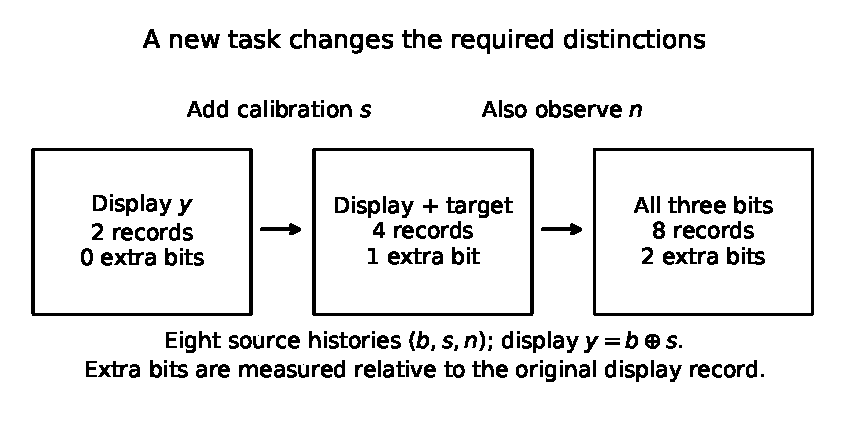
\includegraphics[width=.93\linewidth]{figures/migration_fibres.pdf}
\caption{The required information depends on the revised task. Display alone has two attained values. Adding the target bit requires four joint values. Adding the nuisance bit requires eight. Calibration supplies the first missing distinction, not the second.}\label{fig:migration-fibres}
\end{figure}

\section{Certificates after a change of contract}
A migration map transports data. A certificate authorizes a conclusion only relative to its premises. To reuse a certificate across a revision, specify an old predicate $\varphi$ on $U_0$, a new predicate $\psi$ on $V_0$, and a proved implication
\[
 \varphi(u)\ \Longrightarrow\ \psi(Ju).
\]
An old witness for $\varphi(u)$ and this implication then yield the new conclusion. The implication may express semantic preservation, a stronger guard, or a deliberately weaker postcondition. It cannot be replaced by equality of file names or by an unchanged serialization format.

Chapter~\ref{ch:revision} handles the dependency graph needed to know which such implications remain applicable. The present chapter handles information loss and operation transport. Together they separate three questions that a revision must answer: can the new record be recovered, does it support the required operations, and do the old proof premises still justify the intended conclusions?

\part{Proof and interpretation}
\chapter{Proof fields, closure, and executable certificates}\label{ch:prooffields}

A reasoning archive contains more than its final proofs. It may retain alternative derivations, conjectures, unsuccessful proposals, and observations that later become obsolete. A checker must know which of those records it is permitted to use. Otherwise an archive that is useful for discovery can become an unsound source of premises.

Proof-Path Theory supplies a finite distinction between the surrounding field and the certified derivation. This chapter admits its closure and trace-checking results in a self-contained form. It does not identify acceptance of a data structure with truth of an arbitrary sentence attached to that structure.

\section{A finite field with explicitly admitted rules}
Let $V=\{0,\ldots,n-1\}$ be a finite set of claim addresses. Let $A\subseteq V$ be admitted leaves, $S\subseteq V$ positive observations, and $N\subseteq V$ forbidden consequences. These sets need not be disjoint. A finite rule list $R$ has rows
\[
 r_j=(P_j,c_j),\qquad P_j\subseteq V,\quad c_j\in V.
\]
Only admitted rules are included. Identical rows may occupy different addresses. A conjectural rule elsewhere in the discovery archive is not admitted merely because it has a convenient conclusion.

A model of the field is a set $B\subseteq V$ containing $A$ and satisfying every implication $P_j\subseteq B\Rightarrow c_j\in B$. A protected extension also contains $S$ and avoids $N$. Define
\[
 C_0=A\cup S,\qquad
 C_{k+1}=C_k\cup\{c_j:P_j\subseteq C_k\}.
\]
The terms increase and lie in $V$, so the sequence stabilizes. Write $C$ for its stable value.

\begin{proposition}[The least seeded model]\label{r:field-closure}
The set $C$ is the least model containing $S$. There are at most $n-|A\cup S|$ strict expansion rounds. A protected extension exists if and only if $C\cap N=\varnothing$.
\end{proposition}
\begin{proof}
At a fixed point every enabled rule has its conclusion in $C$, so $C$ is a model containing the seeds. If $B$ is any other model containing $S$, induction gives $C_k\subseteq B$: the seeds lie in $B$, and every rule enabled on $C_k$ has its conclusion in $B$. Hence $C\subseteq B$. Each strict expansion adds at least one of the finitely many nonseed nodes, giving the bound. If $C$ avoids $N$, it is itself a protected extension. If it meets $N$, every seeded model contains that forbidden node, so no protected extension exists.
\end{proof}

A cycle does not create a seed. With rules $u\to v$ and $v\to u$ and no admitted leaves or observations, the least model is empty. The set $\{u,v\}$ is closed, but its members have no derivation from the empty seed. This is why closedness alone is not an adequate proof certificate.

\section{Replay checks a finite causal sequence}
A trace $\sigma=(j_1,\ldots,j_m)$ lists rule addresses. Start from $K_0=A\cup S$. At each step, reject an unknown rule address or a rule whose premises are not all in the current known set. Otherwise adjoin its conclusion. \emph{Strict replay} also rejects a conclusion already known. \emph{Causal replay} allows it.

The distinction concerns the certificate's contract, not the truth of a repeated conclusion. Strict replay records a sequence of new insertions. Causal replay permits reuse of an existing derivation after stronger observations have already supplied one of its intermediate nodes.

\begin{theorem}[Replay is sound and compositional]\label{r:field-replay}
If replay accepts a trace from a set $K\subseteq C$ and returns $K'$, then
\[
 K\subseteq K'\subseteq C.
\]
For either fixed replay mode, replay of a concatenated trace is replay of its first part followed by replay of its second part from the returned set. Failure in either part is failure of the concatenated replay.
\end{theorem}
\begin{proof}
The empty trace changes nothing. At a successful next step, all premises of an admitted rule already lie in $C$. Closedness of $C$ places its conclusion in $C$. Adjoining it preserves the old known set. Induction proves the inclusions. A strict novelty test can reject a step, but does not alter this reasoning for an accepted step.

For concatenation, induct on the first trace. Both computations inspect the same first address, the same current set, and the same enabling and novelty conditions. A rejection ends both computations. A successful step produces identical new sets, after which the induction hypothesis applies.
\end{proof}

\begin{theorem}[Replay and saturation identify exact closure]\label{r:field-exact}
A complete-closure certificate consists of a strict trace and a reported set $B$. Accept it only when replay from $A\cup S$ succeeds with output $B$ and $B$ satisfies every admitted rule. Acceptance implies $B=C$.
\end{theorem}
\begin{proof}
Replay soundness gives $B\subseteq C$. Its extensivity ensures that $B$ contains both seed sets. The saturation check makes $B$ a seeded model, so leastness gives $C\subseteq B$. The two inclusions prove equality.
\end{proof}

The tests serve different purposes. Replay prevents unsupported extra nodes. Saturation prevents omission of a consequence whose rule has not yet been used. Neither test subsumes the other.

\section{A complete negative answer has a witness}
An obstruction certificate contains a forbidden target $v\in N$ and a causal trace deriving $v$ from $A\cup S$.

\begin{theorem}[Finite obstruction witnesses are sound and complete]\label{r:field-obstruction}
An accepted obstruction certificate exists exactly when no protected extension exists. No acyclicity assumption on the rule graph is required.
\end{theorem}
\begin{proof}
An accepted certificate derives a node of $C\cap N$, so Proposition~\ref{r:field-closure} excludes a protected extension.

Conversely, if there is no extension, choose $v\in C\cap N$. Every node in $C$ is reached at a finite stage. Starting with the seeds, process the rules that add the nodes of each successive stage, appending a rule only when its conclusion is not yet known. All its premises belong to an earlier stage and are already known. This yields a finite strict trace reaching the whole closure, and in particular $v$. Its prefix ending when $v$ is first present is also accepted in causal mode. If $v$ is a seed, the empty trace suffices. Cycles cause no difficulty because only rules with already known premises are applied.
\end{proof}

The argument constructs some witness, not a shortest one. Nor does it prove that every implementation of a witness producer terminates or faithfully indexes its source document. A complete result format can require both exact closure and a feasibility flag. A bare negative witness needs only its own replay and forbidden-target check.

\section{A worked four-node certificate}
Let $V=\{0,1,2,3\}$, $A=\{0\}$, $S=\varnothing$, and let the two rules be $0\to1$ and $1\to2$. The exact closure is $\{0,1,2\}$.

The trace containing only the first rule is a valid partial derivation of $\{0,1\}$, but it fails saturation. The set $\{0,1,2,3\}$ is saturated, but node $3$ cannot be produced by replay. The trace of both rules and the exact three-node set pass both tests.

\begin{figure}[htbp]\centering
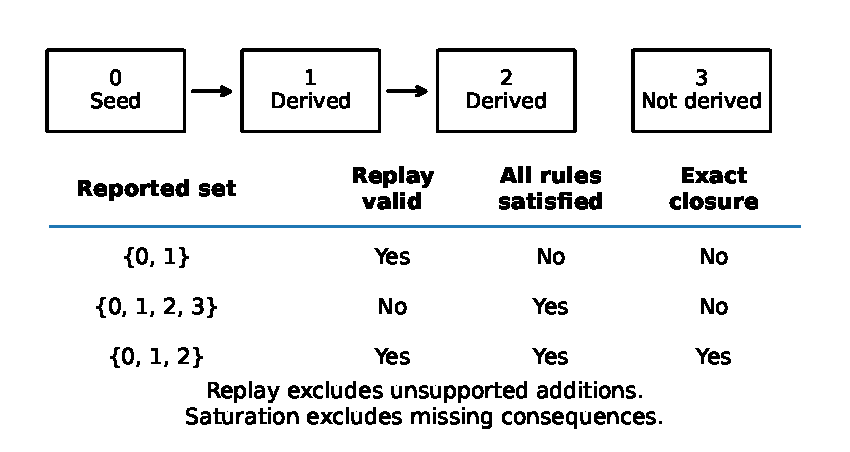
\includegraphics[width=.94\linewidth]{figures/closure_contract.pdf}
\caption{Replay and saturation certify opposite inclusions. A partial derivation omits a consequence. A closed superset can contain an unsupported node. Their conjunction identifies the least seeded model.}\label{fig:closure-contract}
\end{figure}

With forbidden set $N=\{3\}$, the exact closure is a positive feasibility certificate. With $N=\{2\}$, the same closure and the trace to node $2$ certify infeasibility. The request changed, even though the derivation did not. A receiving checker must therefore be given the intended request separately from the producer's proposed answer.

\section{Logical interpretation is an additional map}
Let $\mu(v)$ be the proposition represented by claim address $v$. Suppose every admitted leaf and positive observation is true under $\mu$, and each admitted rule satisfies
\[
 \left(\bigwedge_{p\in P_j}\mu(p)\right)\Longrightarrow\mu(c_j).
\]
Then every node in $C$ is true under $\mu$. Indeed, induction over the closure stages propagates truth from the seeds through the admitted implications.

The finite checker proves derivability relative to those inputs. It does not establish the truth of an empirical observation merely because that observation is placed in $S$. A node excluded by a protected request is likewise not necessarily a logically false proposition. Its appearance shows incompatibility with that request, whose meaning must be stated separately.

\section{The serialization and implementation boundary}
An exchange format must distinguish a problem from its proposed certificate, preserve rule addresses, and reject malformed node identifiers. In Python, for example, a Boolean passes a broad integer-instance test. An address decoder that intends exact integer tokens must exclude that case explicitly. Parsing, range checking, replay, saturation, and interpretation are separate operations.

The Proof-Path Theory source supplies typed problem and certificate records, proved encoder/decoder round trips, an executable Lean replay function, and an accepted-answer theorem at the Lean JSON syntax-tree boundary. Its text parser, file operations, Python implementation, and adapter from named source claims remain separate assurance layers. This chapter uses the finite closure and replay statements, not a blanket verification claim for that entire path.

\source{Proof-Path Theory [PPT], ``Executable certificates for the declared closure,'' ``Finite witnesses for forbidden consequences,'' and ``Typed exchange and the boundary of serialization.'' The selected source statements are \texttt{res:trace:replay}, \texttt{res:trace:least}, \texttt{res:trace:complete}, and \texttt{res:trace:verdict}. Their original formal concordance is preserved with the source excerpt. The present notation and proofs were reviewed as a restatement, not recompiled into a new Lean development.}

\section{Where proof checking enters the reasoning calculus}
The machine-reasoning chain now has a concrete certificate interface. A discovery process can propose a finite derivation without becoming the authority on its validity. The checker verifies the derivation against a fixed problem. A revision can change the problem or its admitted rules, in which case the dependency and migration conditions must be checked again. Reusing the same bytes does not establish that the old certificate answers the new question.

\chapter{Interfaces that remain mathematical research}\label{ch:frontier}

The selected reasoning chain is coherent where its maps share an explicit domain, operational semantics, and evidence language. That does not imply that every proposed component of a machine-native reasoning system has already been joined to every other one. It is useful to state what remains separate, because those boundaries suggest the most precise next theorems.

\section{Existence and acquisition are different problems}
The representation theorems identify when a smaller state \emph{can} preserve selected future observations. They do not generally tell an agent which smaller state to construct from sparse experience. Learning such a state requires a declared hypothesis family, a policy for obtaining observations, and conditions under which incompatible hypotheses can be separated. Statistical identifiability is not certain finite identification. Every finite binary sequence can occur with positive probability under two distinct Bernoulli parameters in $(0,1)$.

A meaningful acquisition result would specify the loss or property of a proposed representation, the permitted query or intervention family, the distribution of observations and the tolerable failure probability. A failure certificate may show the available evidence cannot separate two task-relevant worlds. The resulting impossibility is relative to that evidence interface, not an unconditional impossibility of machine understanding.

\section{A learned semantic map is not a written commuting equation}
Conditional method transport has the form $TF_a=G_{\tau(a)}T$. This is meaningful when $T$, the operator translation $\tau$, and the applicable domains are already specified. A learned system must acquire them, ensure they cover its actual state trajectories, and show the diagrams continue to commute under the relevant interventions. A correct table for a finite declared task is a useful positive control, but it cannot certify that a large recurrent network learned a stable operator language across changed domains.

The Neuralese research documents both finite positive controls and failed stability or scientific gates. Those negative results delimit the next semantic acquisition contracts. An honest mathematical volume keeps the theorem about \emph{given} translators separate from an experiment asking whether one was discovered.

\section{A certificate is not a validated world action}
Chapter~\ref{ch:prooffields} gives the finite closure and replay interface from Proof-Path Theory. Its typed justification fields also distinguish mathematical memory from a completed certificate. A checked proof records a consequence of its premises. Passing a certificate through an executable planning or action system requires additional semantics: which world facts correspond to the propositions, who may perform the selected action, and what actual state change the dispatcher implements.

The Typed Proof Learner and Resolution Completion branches retain relevant constructions, but the recovered handoff does not claim a complete connection from checked propositional derivation to world-action dispatch. Even a fully proved checker theorem would not automatically verify its external parser, message transport, or control interface. Those are additional refinement obligations.

\section{Revision requires dependency completeness}
A revision may change the observation vocabulary, the task, the permitted actions, the model family or the representation used to express an old result. The statement of a theorem can remain true while its application becomes invalid. A retained dependency graph makes selective invalidation possible if the graph is complete for the applicable premises. Matching a recorded digest checks an integrity claim about bytes under its hashing assumptions. It does not establish the adequacy of the recorded dependency set.

Chapter~\ref{ch:migration} gives an exact criterion for migrating finite records and transporting common operations. A broader revision theorem must additionally carry a translation of certificate premises and prove that every retained conclusion remains justified when the model, evidence language, and allowed operations change together. In the absence of those data, an old result should remain accessible as historical mathematics but should not automatically authorize a new action. Formalizing that rule is more valuable than assigning another name to a ``self-correcting agent.''

\section{Resources, workspaces, and authority}
Improvement claims also require a common cost ledger. Reduced operator calls may be outweighed by the preparation, validation or storage needed to obtain a reusable method. Different price weights can change the sign of a proposed saving even when semantic correctness remains unchanged. The reviewed core already formalizes a finite version of this principle. Broad claims of scalable or indefinite improvement require additional assumptions about task distributions, resource limits and repeated acquisition.

Likewise, jointly reconstructible information is not sufficient for a functioning workspace or a machine society. Causal relevance, persistence, identity, access rules, permissions, institutional formation and accountable endings require their own theorems. The safe-ending calculation of Chapter~\ref{ch:endinganalysis} uses a stipulated action system. It does not show that authority was legitimately established or that real institutions will comply with a command.

\section{A bounded agenda}
The strongest next steps are mathematical and testable. Complete the four selected Lean correspondence targets. Extend the exact migration and support-enclosure contracts to revisions of observation models and certificate semantics. Add explicit no-go examples for proposed learned semantic translators when an observation interface is insufficient. Then establish restricted refinement theorems linking a certificate checker to a producer and to a declared runtime, rather than promising end-to-end verification of every historical component. These are substantial research tasks, but each admits finite exact examples, sharp hypotheses and ordinary mathematical review before any large-scale training campaign.

\backmatter
\chapter{Glossary}
\begin{multicols}{2}
\small
\begin{description}[style=nextline,itemsep=3pt,parsep=0pt]
\item[Realization] A compatible family of typed views meeting declared restriction constraints, or a concrete mathematical model satisfying a specified system contract.
\item[Representation] A map or retained record together with the questions and operations it is required to preserve.
\item[Evidence] Information accessible through declared observation or intervention protocols, not an assumed hidden truth label.
\item[Predictive closure] Existence of an update on retained state that commutes with the protected dynamics.
\item[Packet] A typed resolved component or projection. It is not automatically a probability distribution.
\item[Residual] A discrepancy relative to a specified representation or operation contract. Its interpretation depends on the chosen norm or invariant.
\item[Correction signature] A retained equivalence class preserving the outcomes of all allowed future evidence filters on the target.
\item[Instrument] A joint next-state and report probability law, including the evidence scale needed for normalization.
\item[Legal-operation quotient] An abstraction preserving labels, action availability and successor semantics on all enabled actions.
\item[Certificate] Typed evidence for a named mathematical or operational claim relative to its explicit assumptions.
\item[Proof field] The larger network of typed claims and justifications within which a certified proof is located.
\item[Ending attractor] States from which a sure ending is possible under all admitted successor choices.
\item[Running kernel] The greatest region invariant under some running strategy that preserves immediate membership in the ending attractor.
\item[Attained domain] The image of an actual record map. A decoder on attained values does not assign meaning to impossible records.
\item[Conservative envelope] A model that includes every possible actual successor and admits only actions available throughout the represented fine states.
\item[Migration] A map from a retained old record to a specified new record, with separate conditions for continued operation and certificate reuse.
\item[Seeded closure] The least set containing the admitted leaves and observations and closed under every admitted rule.
\item[Strict replay] A trace check requiring each accepted rule step to add a new conclusion.
\item[Causal replay] A trace check that allows already known conclusions, while still requiring every premise at the time of use.
\item[Assurance boundary] The precise source, computation, proof environment, or external premise supported by a verification record.
\end{description}
\normalsize
\end{multicols}
\chapter{Proof and verification guide}\label{app:verification}

\section*{Three levels of evidence}
A written proof establishes a conditional mathematical argument. An exact reference computation exercises specified finite inputs and checks an implementation against a declared oracle. A Lean certificate checks a formal declaration in a particular environment. The correspondence between the English statement and that declaration is an additional mathematical obligation.

The selected core contains twenty-seven numbered theorem, proposition, and corollary statements. Its archived Machine Theory correspondence accepts twenty-three of them in specified scopes. The four remaining selected targets are Theorem~\ref{r:common}, Proposition~\ref{r:positive-packets}, Corollary~\ref{r:occupancy}, and Theorem~\ref{r:ending}. The expanded ending argument does not change that status.

The new composition, control-transport, and migration statements have written proofs and exact finite reference checks. They have not been compiled as new Lean declarations. The proof-field chapter restates selected results from Proof-Path Theory, whose original definitions have an archived formal concordance. That source evidence is retained separately and is not counted as additional coverage of the twenty-seven-result core.

\section*{Scope of the archived core correspondence}
The retained source record reports two completed builds from empty local object directories, including one from a separately extracted source snapshot. Each build compiled sixty-four production modules, replayed sixty-three substantive modules through Lean's own kernel, and checked the declared negative controls and axiom policy. The source inventory contains 1,003 authored theorem declarations supporting the twenty-three selected source results. Supporting declarations and manuscript results are different counts.

The stated foundational axiom set is \texttt{propext}, \texttt{Classical.choice}, and \texttt{Quot.sound}. The upstream compiler and dependency cache are part of the trust boundary. The archive records their identities but does not establish an independently implemented kernel or a new rebuild of all upstream mathematics. No fresh Lean compilation is claimed for the present continuation.

\section*{Exact computational checks}
The reproducibility companion retains the reference programs, input domains, outcomes, and hashes. The following rows use different units and should not be added into a single theorem or evidence count.

\small
\begin{longtable}{@{}p{.27\linewidth}p{.22\linewidth}p{.43\linewidth}@{}}
\toprule Suite & Recorded scope & What is compared\\\midrule\endhead
Reviewed-core regressions & 205,477 assertions in 27 groups & The two original exact suites, retained unchanged and rerun.\\[3pt]
Safe continuation & 8,306 finite games & Fixed-point regions against explicit positional-policy enumeration, with ending-rank witnesses.\\[3pt]
Joint stochastic/legal interface & Four scenarios, horizons zero through four & Complete projected state paths, labels, action/report histories, positive-history posteriors, and action intersections.\\[3pt]
Controlled quotient transport & 5,604 exact quotient cases & Predecessor identities, both fixed-point sequences, ending ranks, and lifted positional witnesses.\\[3pt]
Conservative support envelopes & 3,000 constructed cases & One-sided containment of ending and running regions under adversarial overapproximation.\\[3pt]
Record migration & 44,168 canonical record pairs & Fibre criteria, supplementary encodings, and smaller exhaustive domains for explicit decoders, observations, and operation transport.\\[3pt]
Proof fields & 42,560 protected requests & Closure and feasibility against enumeration of all seeded closed models in the stated small domains.\\\bottomrule
\end{longtable}
\normalsize

The joint-interface checker retains every intermediate state. Comparing only a final state together with an action/report word would not establish full label-history equality. The control checks also distinguish an empty action catalogue from an action with an empty successor set. The latter is rejected, rather than accepted by a vacuous universal condition.

Seeded larger games are exact computations on sampled finite fixtures. They are not exhaustive coverage of all games of those sizes. All probability calculations in the joint-history checks use rational arithmetic. Plotting converts declared exact quantities into display coordinates only.

\section*{Remaining formal obligations}
The next selected target is the sure-ending and safe-running equivalence. A source-facing port must include finite stabilization, first-entry ranks, deadlock, necessity for history-dependent strategies, and the observable command boundary. The common observable quotient must include switching candidate dynamics. The packet result must retain the cone and zero-mass hypotheses. The correction-memory result must retain the full declared evidence algebra and the exact cardinality statement.

No broader claim follows merely from completing those four mappings. The joint controlled-history theorem, the support-game interface, and representation migration have their own future correspondence obligations. Independent mathematical review, native-platform execution, and external validation of learned or physical models are also separate from the checks described here.


\chapter{Result and source map}\label{app:map}
The following map gives the role of each selected written result. Exact source anchors, excerpts, hashes, and detailed hypothesis review are in the accompanying machine-readable ledger and review files. Source relationships do not imply that every source page is admitted.
\small
\begin{longtable}{p{0.13\linewidth}p{0.39\linewidth}p{0.35\linewidth}}
\toprule Result & Preserved object & Source relationship\\\midrule\endhead
\ref{r:factor} & A target determined by an available record & GA, shared fibre criterion.\\
\ref{r:behavior} & Every declared finite continuation & GA and MU, consolidated.\\
\ref{r:packet} & Exact split encoding and named composition loss & SR, split and hidden-return identities.\\
\ref{r:transport} & Source operations and matched readouts & MU, with related uses in OSL and Neuralese use the same conditional principle.\\
\ref{r:common} & One output method across candidate dynamics & GA, common observable quotient.\\
\ref{r:positive-packets} & Probability interpretation of a complete packet family & LSM, positive packet criterion.\\
\ref{r:memory} & Every admitted future set correction & GA, correction-signature theorem.\\
\ref{r:occupancy} & Exact partition-evidence memory cardinality & GA, occupancy corollary.\\
\ref{r:bayes} & All posterior updates in the actual reporting chain & MU, finite channel factorization.\\
\ref{r:joint-refinement} & Coarsest partition closed for prediction and update & LSM and PRIQ, finite closure.\\
\ref{r:instrument} & Joint next-state/report law, posteriors and feedback & PRIQ and AVOC, selected composition.\\
\ref{r:history-bound} & Whole-history error and conditioning cost & LSM, law and normalization bounds.\\
\ref{r:risk} & One bounded-loss decision calculation & GA and MU, specialized common-risk bound.\\
\ref{r:recipient} & One artifact under fixed recipient procedures & MU, intersection and covering criterion.\\
\ref{r:inquiry} & One executable tree under all declared budgets & MU and SII, finite Pareto synthesis.\\
\ref{r:lowerbound} & A complete optimality claim for a checked tree & SII, binary singleton-repair scope.\\
\ref{r:belief-planning} & One optimal finite-horizon expected-cost inquiry & AVOC, projected values and finite plans.\\
\ref{r:policy-error} & Uniform policy evaluation before selection & LSM/AVOC, common-law specialization.\\
\ref{r:cegis} & Exact finite candidate rejection and acceptance & SII, finite counterexample refinement.\\
\ref{r:ordered} & The same proposed ASTs and teacher transcript & SII, sound equations and ordered quotient.\\
\ref{r:prefix} & The same completed ordered diagnostic search & SII, capacity and streaming arguments.\\
\ref{r:dependencies} & Applicability of dependency-bound witnesses & SII, complete declared dependency graph.\\
\ref{r:prices} & Gains under one complete additive ledger & SII, price-relative dominance.\\
\ref{r:lineage} & Conditional false-acceptance control & SII, adaptive lineage error budget.\\
\ref{r:reconstruction} & A target from jointly accessible linear records & SR and SRWT, target-relative specialization.\\
\ref{r:governance} & Legal action availability and label histories & MS, exact governance quotient.\\
\ref{r:ending} & Continued operation with an ending policy & MS, fully observed finite specialization.\\\bottomrule
\end{longtable}
\normalsize

\clearpage
\section*{Selected core correspondence}\small
\begin{longtable}{@{}p{.11\linewidth}p{.55\linewidth}p{.25\linewidth}@{}}\toprule Result & Statement & Archived correspondence\\\midrule\endhead
\ref{r:factor} & A record determines a target exactly on its fibres & Accepted, scoped\\
\ref{r:behavior} & Evidence-initialized behavioral state & Accepted, scoped\\
\ref{r:packet} & Exact accounting of the discarded excursion & Accepted, scoped\\
\ref{r:transport} & Forward transport of a reusable method & Accepted, scoped\\
\ref{r:common} & A common observable quotient & Pending\\
\ref{r:positive-packets} & When complete packets are genuine probability components & Pending\\
\ref{r:memory} & Minimal exact memory for a correction contract & Accepted, scoped\\
\ref{r:occupancy} & The size of partition correction memory & Pending\\
\ref{r:bayes} & When a report preserves every Bayesian correction & Accepted, scoped\\
\ref{r:joint-refinement} & Least refinement closed under prediction and correction & Accepted, scoped\\
\ref{r:instrument} & One quotient for reports, posteriors, and feedback & Accepted, scoped\\
\ref{r:history-bound} & A whole-history bound with an explicit conditioning cost & Accepted, scoped\\
\ref{r:risk} & A decision bound for one actual approximation chain & Accepted, scoped\\
\ref{r:recipient} & A common artifact for fixed recipients & Accepted, scoped\\
\ref{r:inquiry} & Exact joint feasibility for explicit controllers & Accepted, scoped\\
\ref{r:lowerbound} & A candidate attaining both lower bounds is optimal & Accepted, scoped\\
\ref{r:belief-planning} & The same compressed belief supports the same inquiry & Accepted, scoped\\
\ref{r:policy-error} & Uniform model error controls a changed policy & Accepted, scoped\\
\ref{r:cegis} & What finite counterexamples establish & Accepted, scoped\\
\ref{r:ordered} & Ordered semantic compression preserves the teacher trace & Accepted, scoped\\
\ref{r:prefix} & A sound prefix exclusion & Accepted, scoped\\
\ref{r:dependencies} & Selective reuse with complete dependencies & Accepted, scoped\\
\ref{r:prices} & Which gains survive every admitted price? & Accepted, scoped\\
\ref{r:lineage} & A conditional error budget for a lineage & Accepted, scoped\\
\ref{r:reconstruction} & Target-relative joint reconstruction & Accepted, scoped\\
\ref{r:governance} & A quotient that preserves legal operations & Accepted, scoped\\
\ref{r:ending} & Safe continuation that retains an ending strategy & Pending\\
\bottomrule
\end{longtable}\normalsize
\chapter{Sources and references}
The named sources below identify the mathematical lineages used in this book. Exact editions, file hashes, source positions, and review records belong to the accompanying source register. A source citation does not import every result or every implementation in that source.

\begin{description}[style=nextline]
\item[KS] Komorebi P. \emph{Komorebi Space: Coherent Realizations, Obstructions, and Descent}. The prologue uses strict coherent families, view evaluation, and attained-record factorization. The full analytic and descent theories are not assumed here.
\item[GA] Komorebi P. \emph{Grounded Abstraction: Identifiability, Representation Change, and the Limits of Learning}. Evidence access, predictive initialization, correction signatures, model uncertainty, and information required for migration.
\item[MU] Komorebi P. \emph{Machine Understanding: Representation, Explanation, and Transfer}. Reusable methods, recipient-relative artifacts, Bayesian reporting, and a common acquisition and resource contract.
\item[SII] Komorebi P. \emph{Self-Improving Intelligence: Representation, Discovery, and Recursive Revision}. Finite discovery, semantic compression, diagnostic pruning, dependency reuse, and resource and lineage bounds.
\item[MS] Komorebi P. \emph{Machine Societies: A Theory of Persistent Plural Computational Organization}. Selected joint-reconstruction, action-quotient, and continuation results. Institutional formation and external authority are not inferred from those finite results.
\item[SR] Komorebi P. \emph{Sufficient Resolution}. Split encodings, hidden-return identities, factorization, and target-relative reconstruction.
\item[SRWT] Komorebi P. \emph{Stratified Relational Workspace Theory}. The selected joint-reconstruction argument is used without importing the complete dynamics, emergence, persistence, or identity theory.
\item[LSM] Komorebi P. \emph{Large Signal Model Foundations}. The selected core's source anchors are the positive-packet criterion, joint prediction/correction closure, and whole-law and conditioning bounds. The source register retains the earlier edition actually used for those anchors, alongside the newer monograph. The larger observable-learning and domain-discovery program remains a separate source.
\item[PRIQ] Komorebi P. \emph{Hypergraph Lumpability and Bayesian Refinement for Dynamical Systems with Projector Resolutions}. Selected positive normalization and finite filtering arguments. The full nonlinear analytic and hyperedge theory is not imported.
\item[AVOC] Komorebi P. \emph{Artifact Value, Guarded Operations, and Calibrated Planning}. Selected conditioning, projected-value, and finite-planning mechanisms. The formal scope of the source implementation is distinct from the source-facing Machine Theory correspondence.
\item[PPT] Komorebi P. \emph{Proof Path Theory: Certificates, Compression, Discovery Fields, and Mathematical Memory}. Seeded closure, replay, obstruction witnesses, and typed certificate exchange. The selected trace-extension source and original formal concordance are retained in the companion.
\item[OSL] Komorebi P. \emph{Operator-Symbolic Language}. Used to identify the executable semantic interface and its remaining learned-translation boundary.
\item[NEU] Komorebi P. \emph{Neuralese: Recurrent Latent Operators, Causal Semantics, and Stability}. Used for its distinction between a specified semantic executor and a learned representation. Historical positive and failed scientific gates retain their original scope.
\item[SRIC] Komorebi P. \emph{Stratified Recursive Improvement Closure: Obstruction, Descent, Transport, and Evidence-Preserving Lineages}. A specialist source for recursive repair and evidence retention, not a blanket claim of unrestricted self-improvement.
\item[KLC] Leslie Pack Kaelbling, Michael L. Littman, and Anthony R. Cassandra. ``Planning and acting in partially observable stochastic domains.'' \emph{Artificial Intelligence} 101 (1998), 99--134. Classical context for belief-state planning and finite policies.
\end{description}

These references are not an exhaustive literature or priority audit. Factorization, automata quotients, sufficient statistics, dynamic programming, program synthesis, closure systems, and controlled invariant sets have established mathematical foundations. The selected arguments are given with their hypotheses so that their use does not depend on an unstated attribution claim.

\section*{Source treatment}
The original reviewed text and formal mappings are preserved separately. This monograph makes local type and domain assumptions explicit, repairs the path-level composition argument, and adds the subsequent integration chapters. The editorial record identifies those changes. Original source-suite runs remain historical evidence unless a new receipt records an actual rerun. The current finite regressions do not establish a fresh source-wide mathematical audit of every specialist manuscript.

\end{document}
